\documentclass[12pt, oneside,a4paper]{article}
\usepackage{ctex}
\usepackage{geometry}
\usepackage{indentfirst}               		
\usepackage{listings}
\usepackage{color}
\usepackage{textcomp}
\definecolor{dkgreen}{rgb}{0,0.6,0}
\definecolor{gray}{rgb}{0.5,0.5,0.5}
\definecolor{mauve}{rgb}{0.58,0,0.82}
\usepackage{amssymb,amsmath}
\usepackage[noend]{algpseudocode}
\usepackage{algorithmicx,algorithm}
\usepackage[font=small,labelfont={bf,sf},tableposition=top]{caption}
\usepackage{graphicx}
\usepackage{multirow}
\usepackage{float}
\usepackage{fancyhdr}
\lstset{frame=tb,
  language=Java,
  aboveskip=3mm,
  belowskip=3mm,
  showstringspaces=false,
  columns=flexible,
  basicstyle={\small\ttfamily},
  numbers=none,
  numberstyle=\tiny\color{gray},
  keywordstyle=\color{blue},
  commentstyle=\color{dkgreen},
  stringstyle=\color{mauve},
  breaklines=true,
  breakatwhitespace=true,
  tabsize=3
}
\geometry{a4paper,left=2cm,right=2cm,top=3cm,bottom=3cm}

\pagestyle{fancy}
\lhead{数据库引论 Project \# 1}
\rhead{胡天晓, 张昊晗, 刘婧源}

\newcommand{\HRule}{\rule{\linewidth}{0.5mm}}
\begin{document}

\begin{titlepage}
\begin{center}
% Upper part of the page
\textsc{\LARGE 复旦大学}\\[1.5cm]
\textsc{\Large 数据库引论}\\[0.5cm]
% Title
\HRule \\[1.0cm]
{ \huge \bfseries Project 1: Glutton}\\[0.4cm]
\HRule \\[1.5cm]

\includegraphics[width=2in]{logo.jpg}\\[1cm]
% Author
\begin{minipage}{0.4\textwidth}
\begin{flushleft} \large
\begin{center}
\emph{小组成员:}\\
胡天晓\\
张昊晗\\
刘婧源
\end{center}
\end{flushleft}
\end{minipage}
\vfill
% Bottom of the page
{\large \today}
\end{center}
\end{titlepage}

\section{项目简介}
\subsection{项目背景}
Glutton是为复旦大学(张江校区)的吃货们设计的外卖网页应用。以Python链接SQL语言,采用web界面作为为前端。面向对象分为商家和用户,支持商家创建、更改、查询、删除菜品;用户查询商家、菜品,创建、更改、删除、评价订单等基本操作。
\subsection{小组分工情况}
成员分工情况具体如下表:
\begin{table}[!h]
\begin{tabular}{|c|c|l|}
\hline
胡天晓 & 14300240007 & 主要负责项目的后端开发(利用Flask框架连接SQLite数据库进行\\
 & & 数据库的增、删、查、改等操作);项目报告的润色及格式调整。 \\
\hline
张昊晗 & 14300240009 & 主要负责前端开发(利用html5,css与boostrap框架)、动态交互及\\
& & 前后端对接(利用jquery实现,并使用sweetalert与facebox插件)。 \\
\hline
刘婧源 & 15307130385 & 主要负责数据库设计,建表;商家、菜品原始数据的收集及插入;\\
 & & 涉及增删改查的部分SQL语句;项目报告主体部分的撰写。\\
\hline
\end{tabular}
\end{table}
\subsection{项目文件列表}
项目文件结构如下:\\
/Glutton \\
\hspace*{1cm}	/app \\
		\hspace*{1cm}\hspace*{1cm}/static \\
		\hspace*{1cm}\hspace*{1cm}\hspace*{1cm}	/css \\
		\hspace*{1cm}\hspace*{1cm}\hspace*{1cm}\hspace*{1cm}		|... \\
		\hspace*{1cm}\hspace*{1cm}\hspace*{1cm}	/img \\
		\hspace*{1cm}\hspace*{1cm}\hspace*{1cm}\hspace*{1cm}		|... \\
		\hspace*{1cm}\hspace*{1cm}\hspace*{1cm}	/js \\
		\hspace*{1cm}\hspace*{1cm}\hspace*{1cm}\hspace*{1cm}		|... \\
		\hspace*{1cm}\hspace*{1cm}/templates \\
		\hspace*{1cm}\hspace*{1cm}\hspace*{1cm}	|... \\
		\hspace*{1cm}\hspace*{1cm}|\_\_init\_\_.py \\
		\hspace*{1cm}\hspace*{1cm}|views.py \\
	\hspace*{1cm}|app.db \\
	\hspace*{1cm}|config.py \\
	\hspace*{1cm}|create\_db.py \\
	\hspace*{1cm}|insert.sql \\
	\hspace*{1cm}|README.md \\
	\hspace*{1cm}|run.py
\subsection{运行方法}
\begin{lstlisting}
   //安装flask及数据库依赖
   $ pip install flask
   $ pip install sqlite3
   //创建数据库
   $ python create_db.py
   \end{lstlisting}
创建好数据库后,在浏览器中输入http://127.0.0.1:5000/即可访问。
\subsection{开发及测试环境}
\begin{itemize}
\item 后端开发环境为macOS 10.12,python版本为2.7。
\item 前端开发环境为macOS 10.10,浏览器版本为Chrome 58.0(64-bit),在safari,Microsoft Edge上前端测试通过。
\end{itemize}
\subsection{flask简介}
Flask是一个使用Python编写的轻量级Web应用框架。其WSGI工具箱采用Werkzeug,模板引擎则使用Jinja2,采用BSD授权。Flask也被称为“microframework”,因为它仅实现简单的核心,选择用extension来增加其他功能。Flask没有默认使用的数据库和窗体验证工具等,然而由于其保留了扩增的弹性,可以用Flask-extension加入必备的功能。
\subsection{SQLite简介}
SQLite是一款轻型数据库,包含在一个相对小的C库中。它占用资源非常的低,支持Windows/Linux/Unix等等主流操作系统。不像常见的客户-服务器范例,SQLite引擎不是个程序与之通信的独立进程,而是连接到程序中成为它的一个主要部分。整个数据库都在宿主主机上存储在一个单一的文件中,免去了在团队协同开发时数据库迭代带来的重新配置的繁琐。
SQLite的轻量特性十分适合我们的项目,因此我们使用其最新版本SQLite 3作为应用的后端数据库,在python代码中嵌入SQL语句来操作数据库。
Flask十分适合于小型项目的快速开发,因此我们选择用Flask框架来搭建应用的后台部分。
\subsection{前端简介}
Jquery是一个快速、简洁的JavaScript框架,是继Prototype之后又一个优秀的JavaScript代码库。Html5是万维网的核心语言、标准通用标记语言下的一个应用超文本标记语言(HTML)的第五次重大修改。Bootstrap是Twitter推出的一个用于前端开发的开源工具包,是一个CSS/HTML框架,优雅美观。因此我们使用Html5作为前端文本标记语言,css与bootstrap作为样式设计语言,Jquery实现动态效果及前后端对接,并使用了sweetalert,facebox等插件优化动态交互。


\section{项目细节}
 \subsection{针对用户的功能}
我们的web app面向张江地区的吃货。主界面的最上方是导航栏——左侧有四个按钮:可以选择以用户或商家身份使用这个应用;在登录后,还可以查看自己的主页和订单。右侧和中部同为登录和注册按钮。最下方包含了作者、版权信息等。
 \begin{figure}[H]
   \centering
     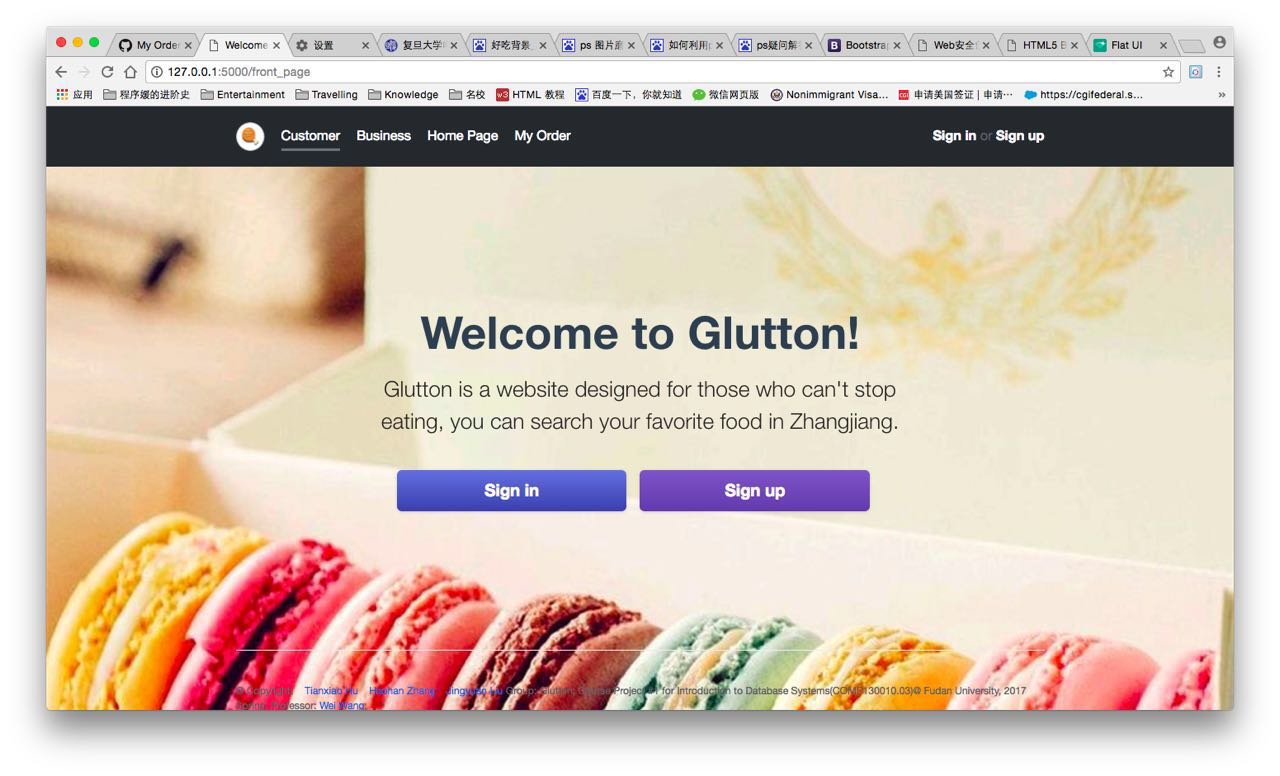
\includegraphics[width=6.00in]{cu-front.jpg}
     \caption{\small{主页面}}
  \end{figure}
  \begin{itemize}
  \item 注册/登录\\
  点击sign up按钮可以进入注册页面,输入用户名,手机号,密码来注册。手机号必须是唯一的,如果有重复,系统会提示这个手机号已经被注册,请直接登录。\\
  点击sign in按钮可以进入登录页面,作为食客需要用手机号和密码登录。如果密码输入错误,系统会提示密码或用户名错误。
  用户在数据库中的密码通过md5方式加密。MD5是一个安全的散列算法,输入两个不同的明文不会得到相同的输出值,根据输出值,不能得到原始的明文,即其过程不可逆;所以要解密MD5没有现成的算法,只能用穷举法,把可能出现的明文,用MD5算法散列之后,把得到的散列值和原始的数据形成一个一对一的映射表,通过比在表中比破解密码的MD5算法散列值,通过匹配从映射表中找出破解密码所对应的原始明文。
  \begin{figure}[H]
   \begin{minipage}[t]{0.5\linewidth}
    \centering
     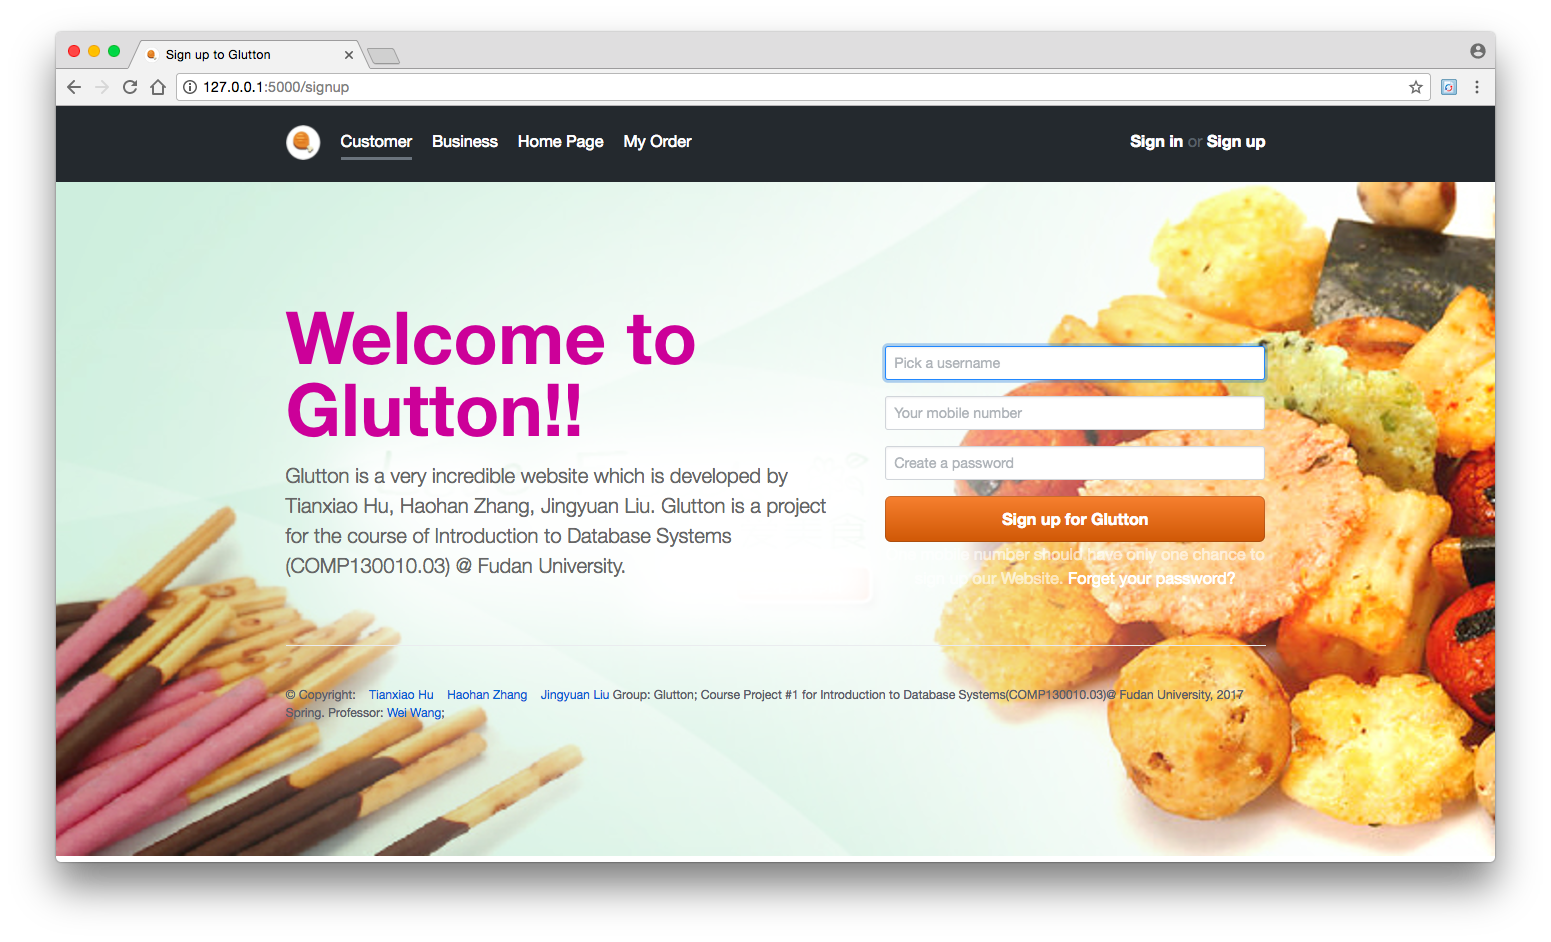
\includegraphics[width=3in]{cu-signup.jpg}
     \caption{\small{用户注册}}
   \end{minipage}
   \begin{minipage}[t]{0.5\linewidth}
    \centering
     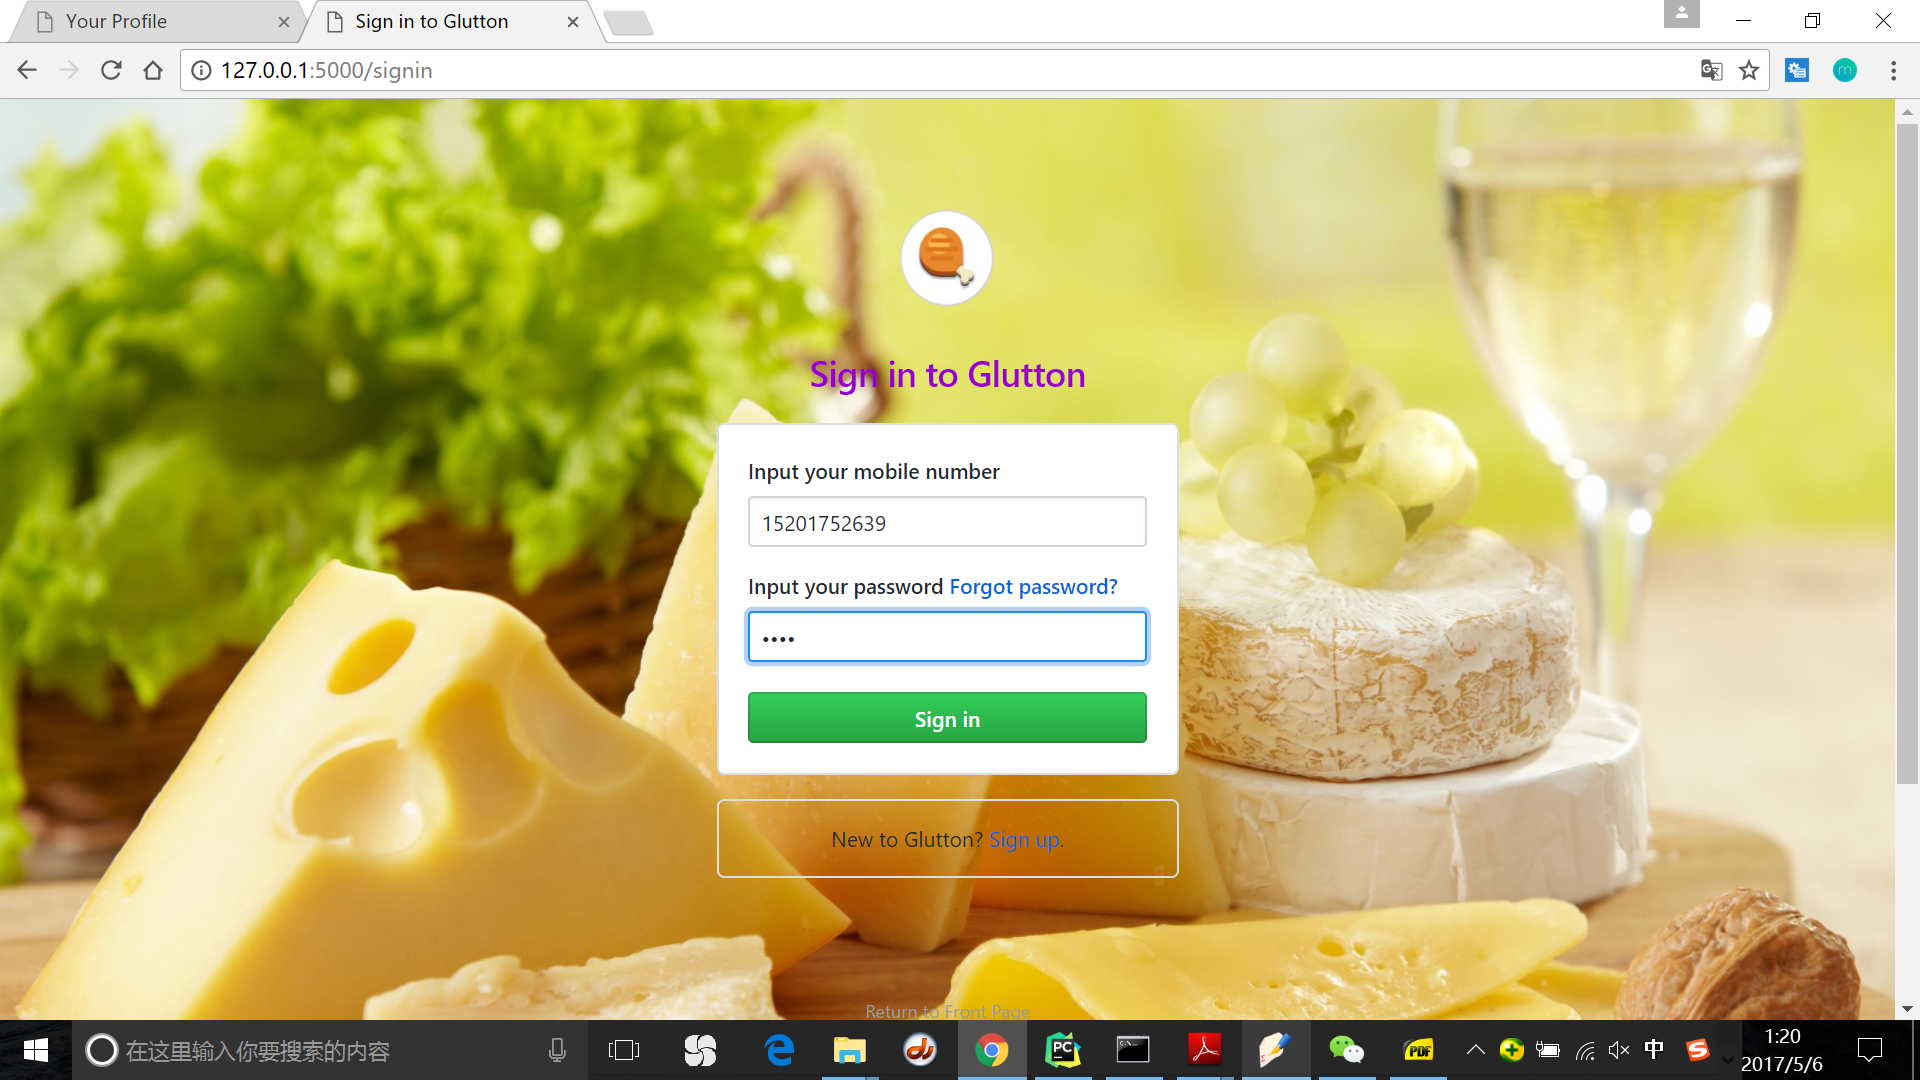
\includegraphics[width=3in]{cu-signin.jpg}
      \caption{\small{用户登录}}
   \end{minipage}
   \end{figure}
  \item 更改信息/头像\\
  登录成功后,我们进入到用户的主页。主页的最上方是导航栏,左侧三个按钮可以选择主页,个人信息,订单。右侧有搜索栏和退出登录按钮。\\
  左侧图片点击可以更改个人口味偏好,下方显示用户名和手机号,以及编辑个人信息按钮。中间同样有搜索栏,下方按食物分类配备了多种类型,如果汁奶茶、炸鸡汉堡等的食物分区,代表性商家可以直接通过鼠标点击进入。\\
    点击Edit profile可以进入修改个人信息页面,左侧可以选择更改的类型:个人口味偏好,基本信息,更改密码,退出登录。\\
  基本信息可以修改用户名、地址、称呼和个人描述;密码修改,如果修改成功,系统会提示“Succeed”

  \begin{figure}[H]
   \begin{minipage}[t]{0.5\linewidth}
    \centering
     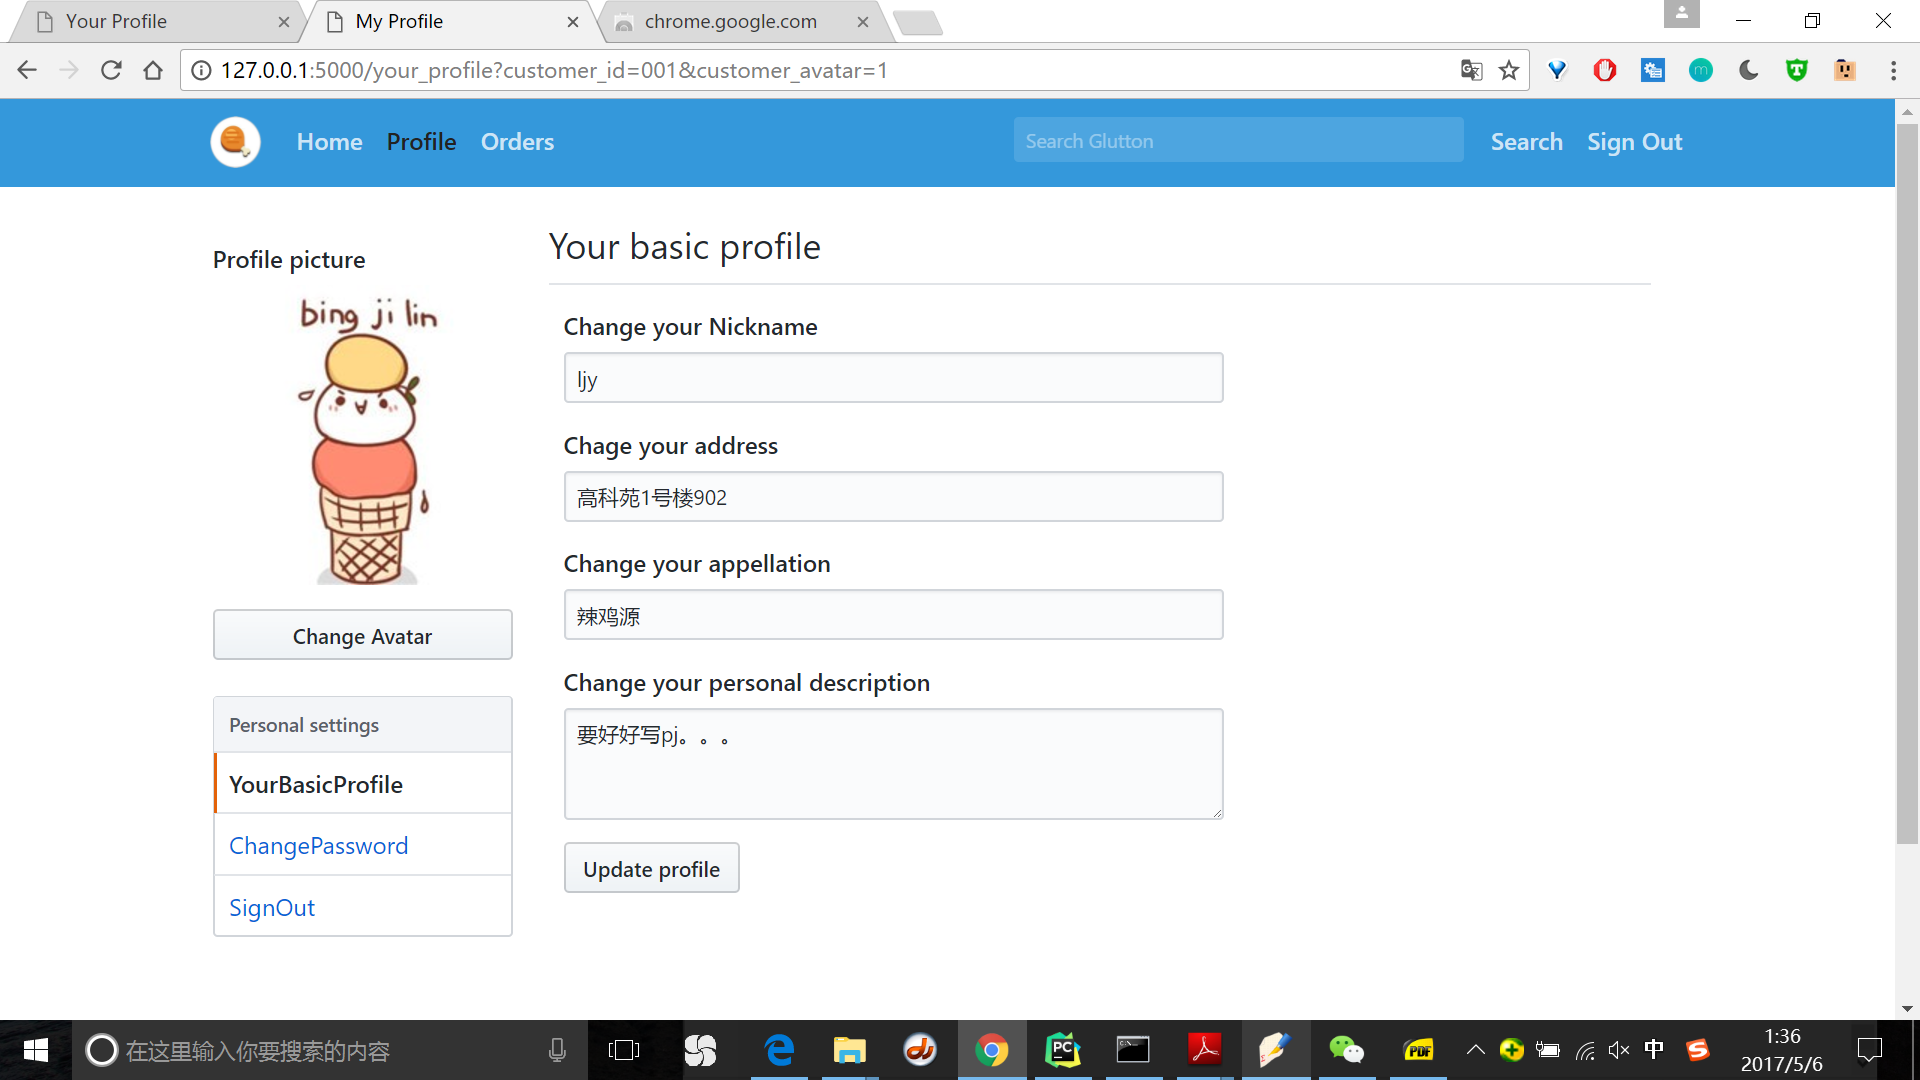
\includegraphics[width=3in]{cu-profile.jpg}
     \caption{\small{用户更改信息}}
   \end{minipage}
   \begin{minipage}[t]{0.5\linewidth}
    \centering
     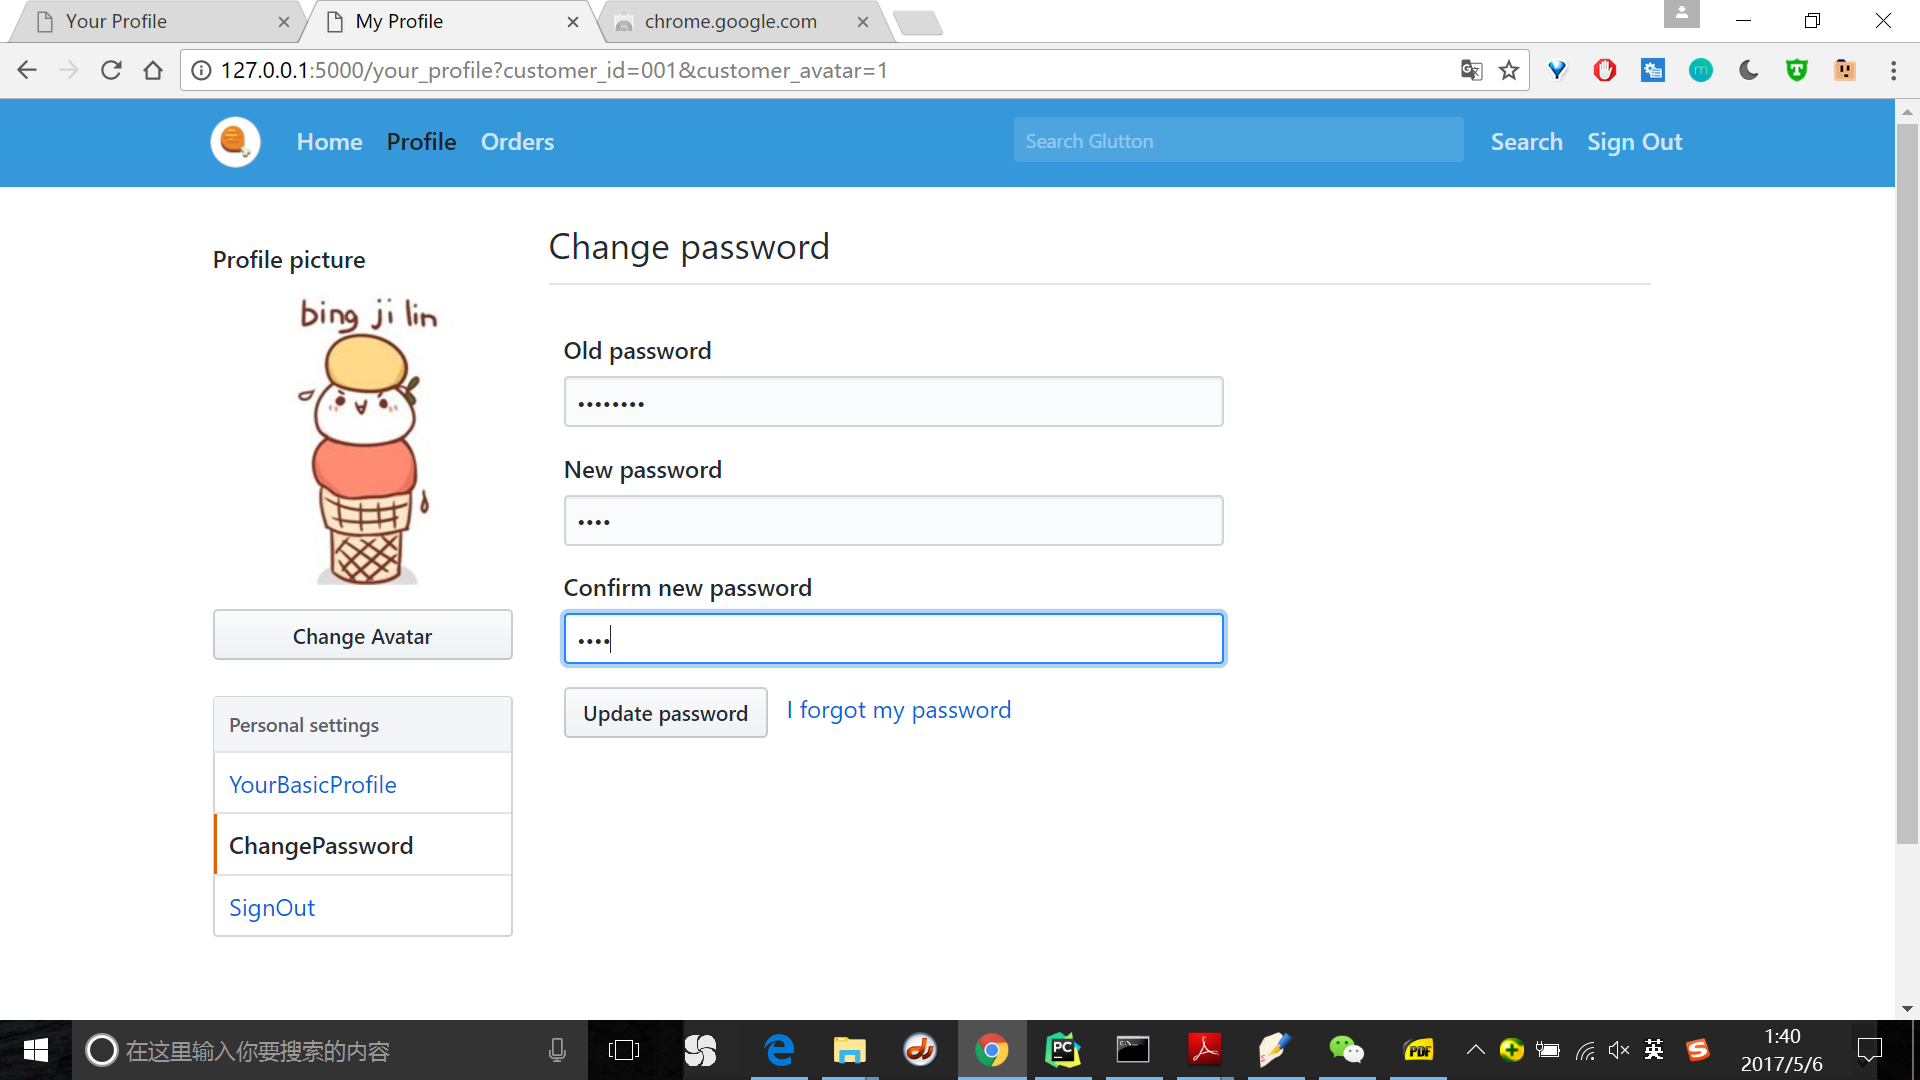
\includegraphics[width=3in]{cu-password.jpg}
      \caption{\small{用户更改密码}}
   \end{minipage}
   \end{figure}

  \begin{figure}[H]
   \centering
     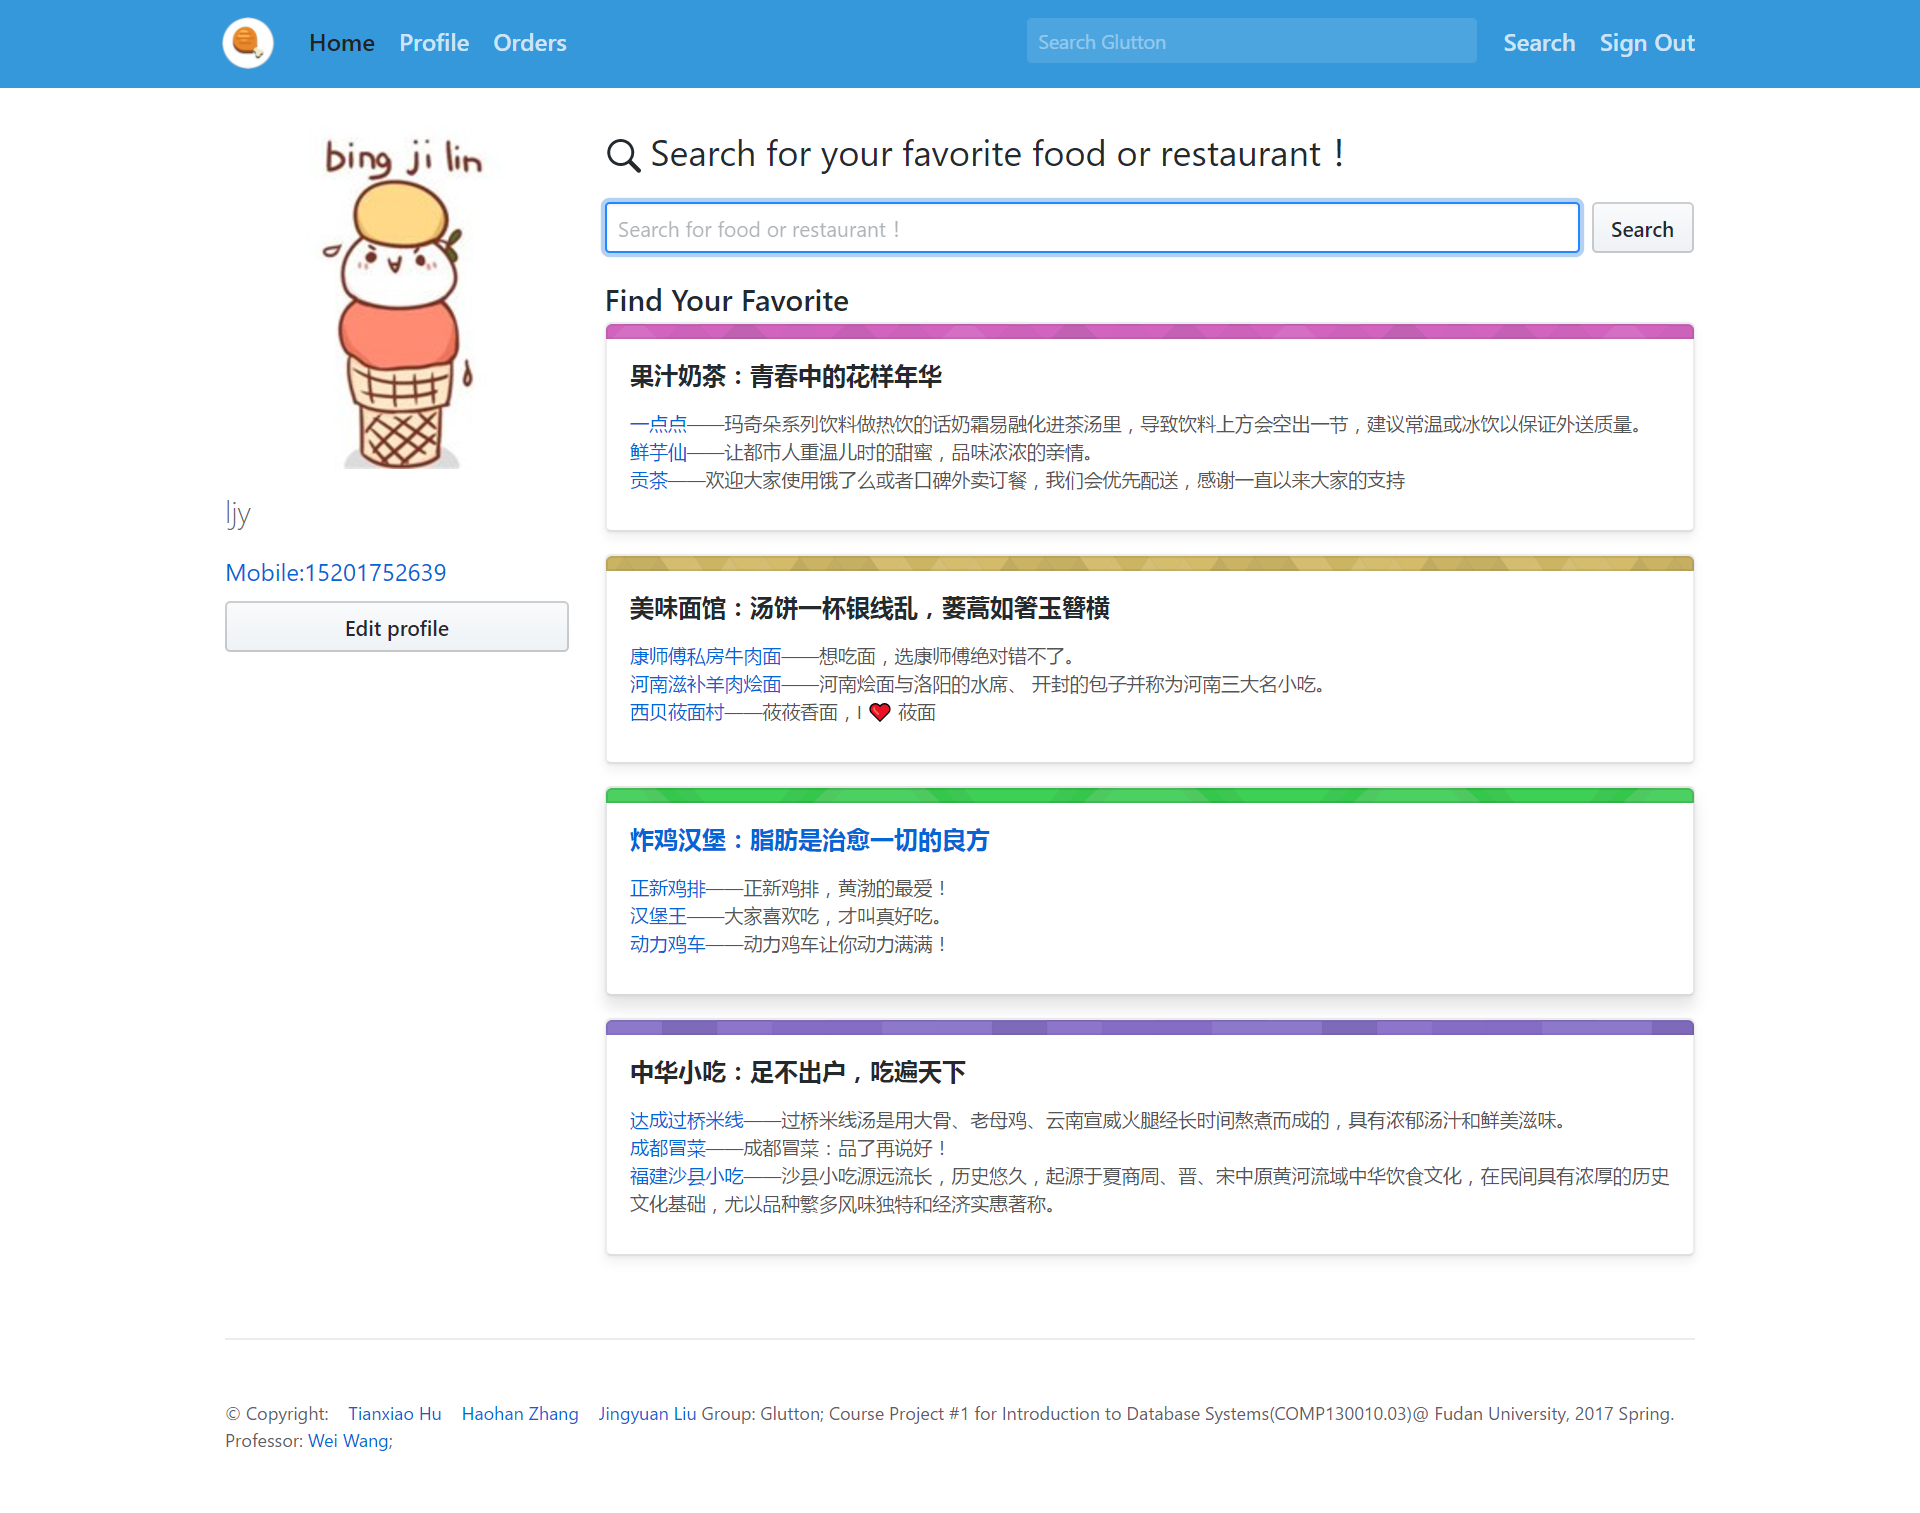
\includegraphics[width=6.00in]{cu-home.png}
     \caption{\small{用户主页}}
  \end{figure}


   用户可以点击图片,修改个人头像。共有九种头像可供选择,随意点击一个用户头像,系统会提示转换成功,页面跳转至个人主页,可以看到用户头像已有变化。
   \begin{figure}[H]
   \centering
     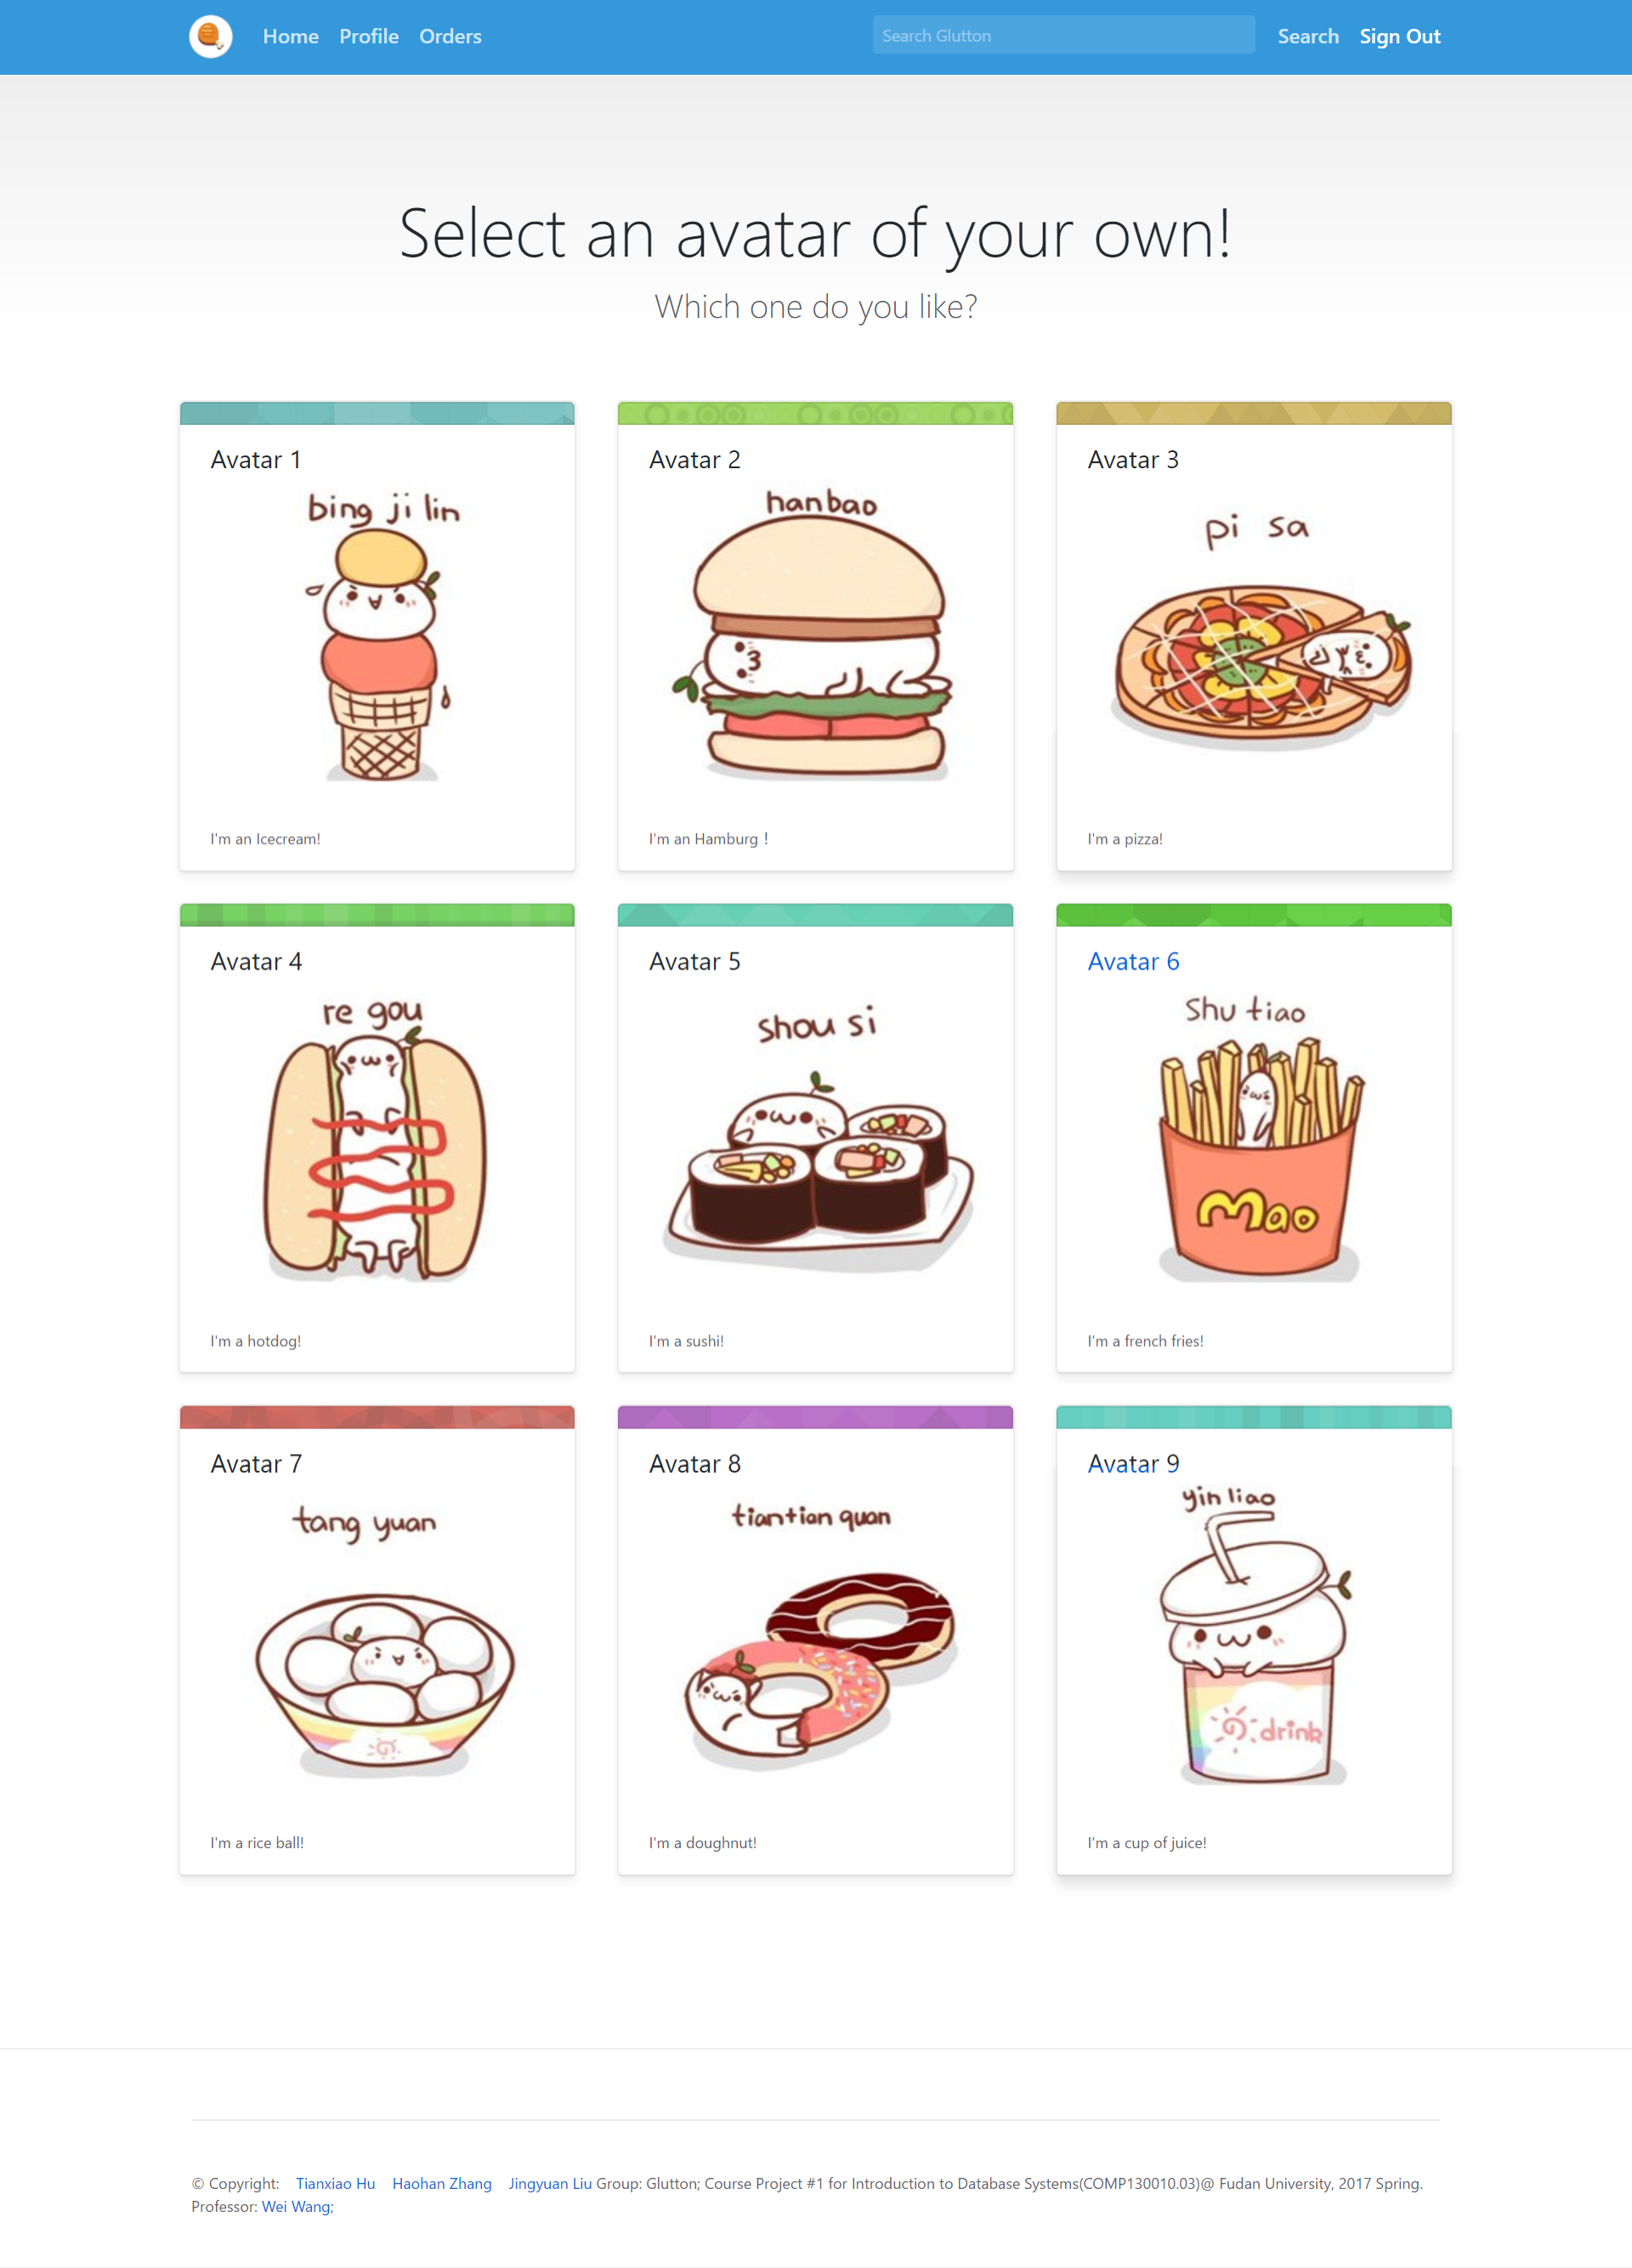
\includegraphics[width=6.00in]{avatar.png}
     \caption{\small{用户头像选择}}
  \end{figure}
  \item 查找商家\\
  在搜索框中输入商家的名称,例如“一点点”,可以查询到对应商家信息。点击可以进入商家。\\
  还可以按照随机、月销量、起送费顺序查看商家列表,右侧有查询历史记录。\\
  同样在商家内,可以按照随机、月销量、商品价格顺序查看菜品列表。
  \begin{figure}[H]
   \centering
     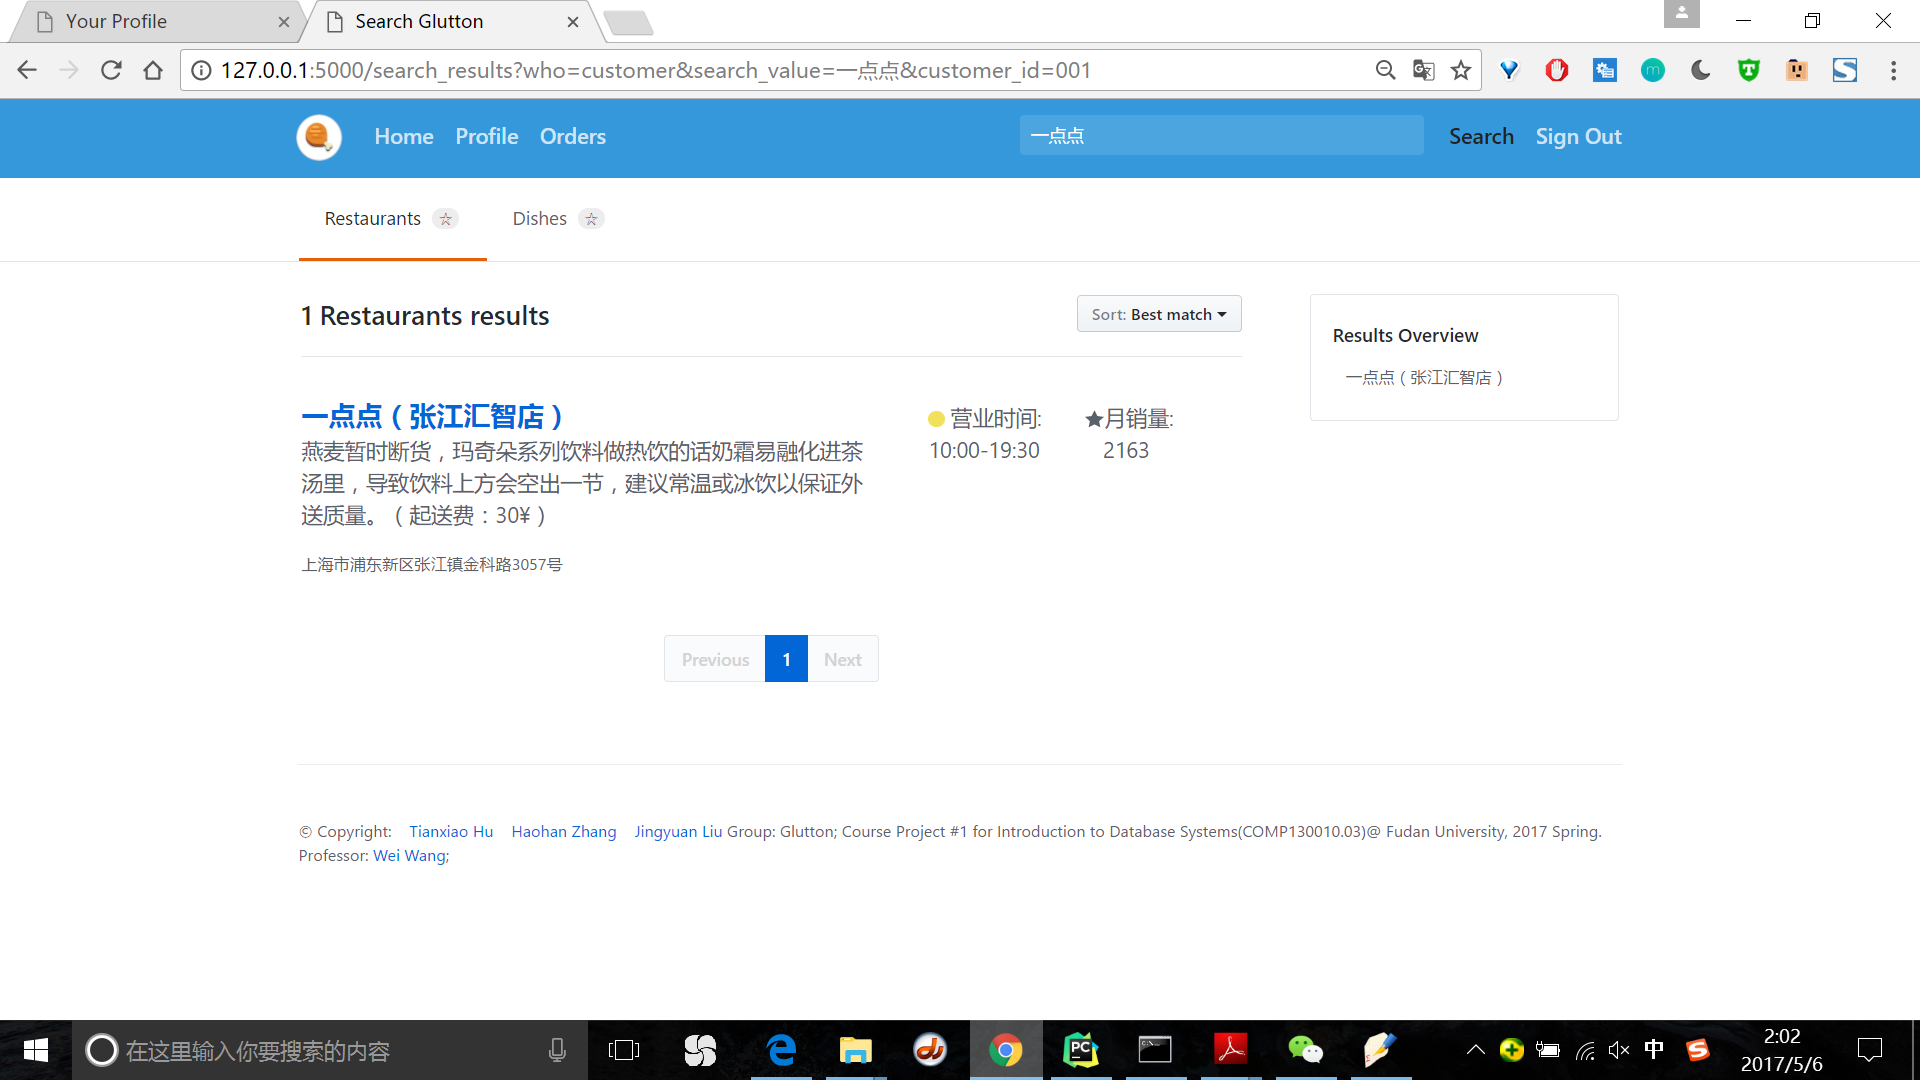
\includegraphics[width=6.00in]{cu-se-re.jpg}
     \caption{\small{用户查找特定商家}}
  \end{figure}
  \begin{figure}[H]
   \centering
     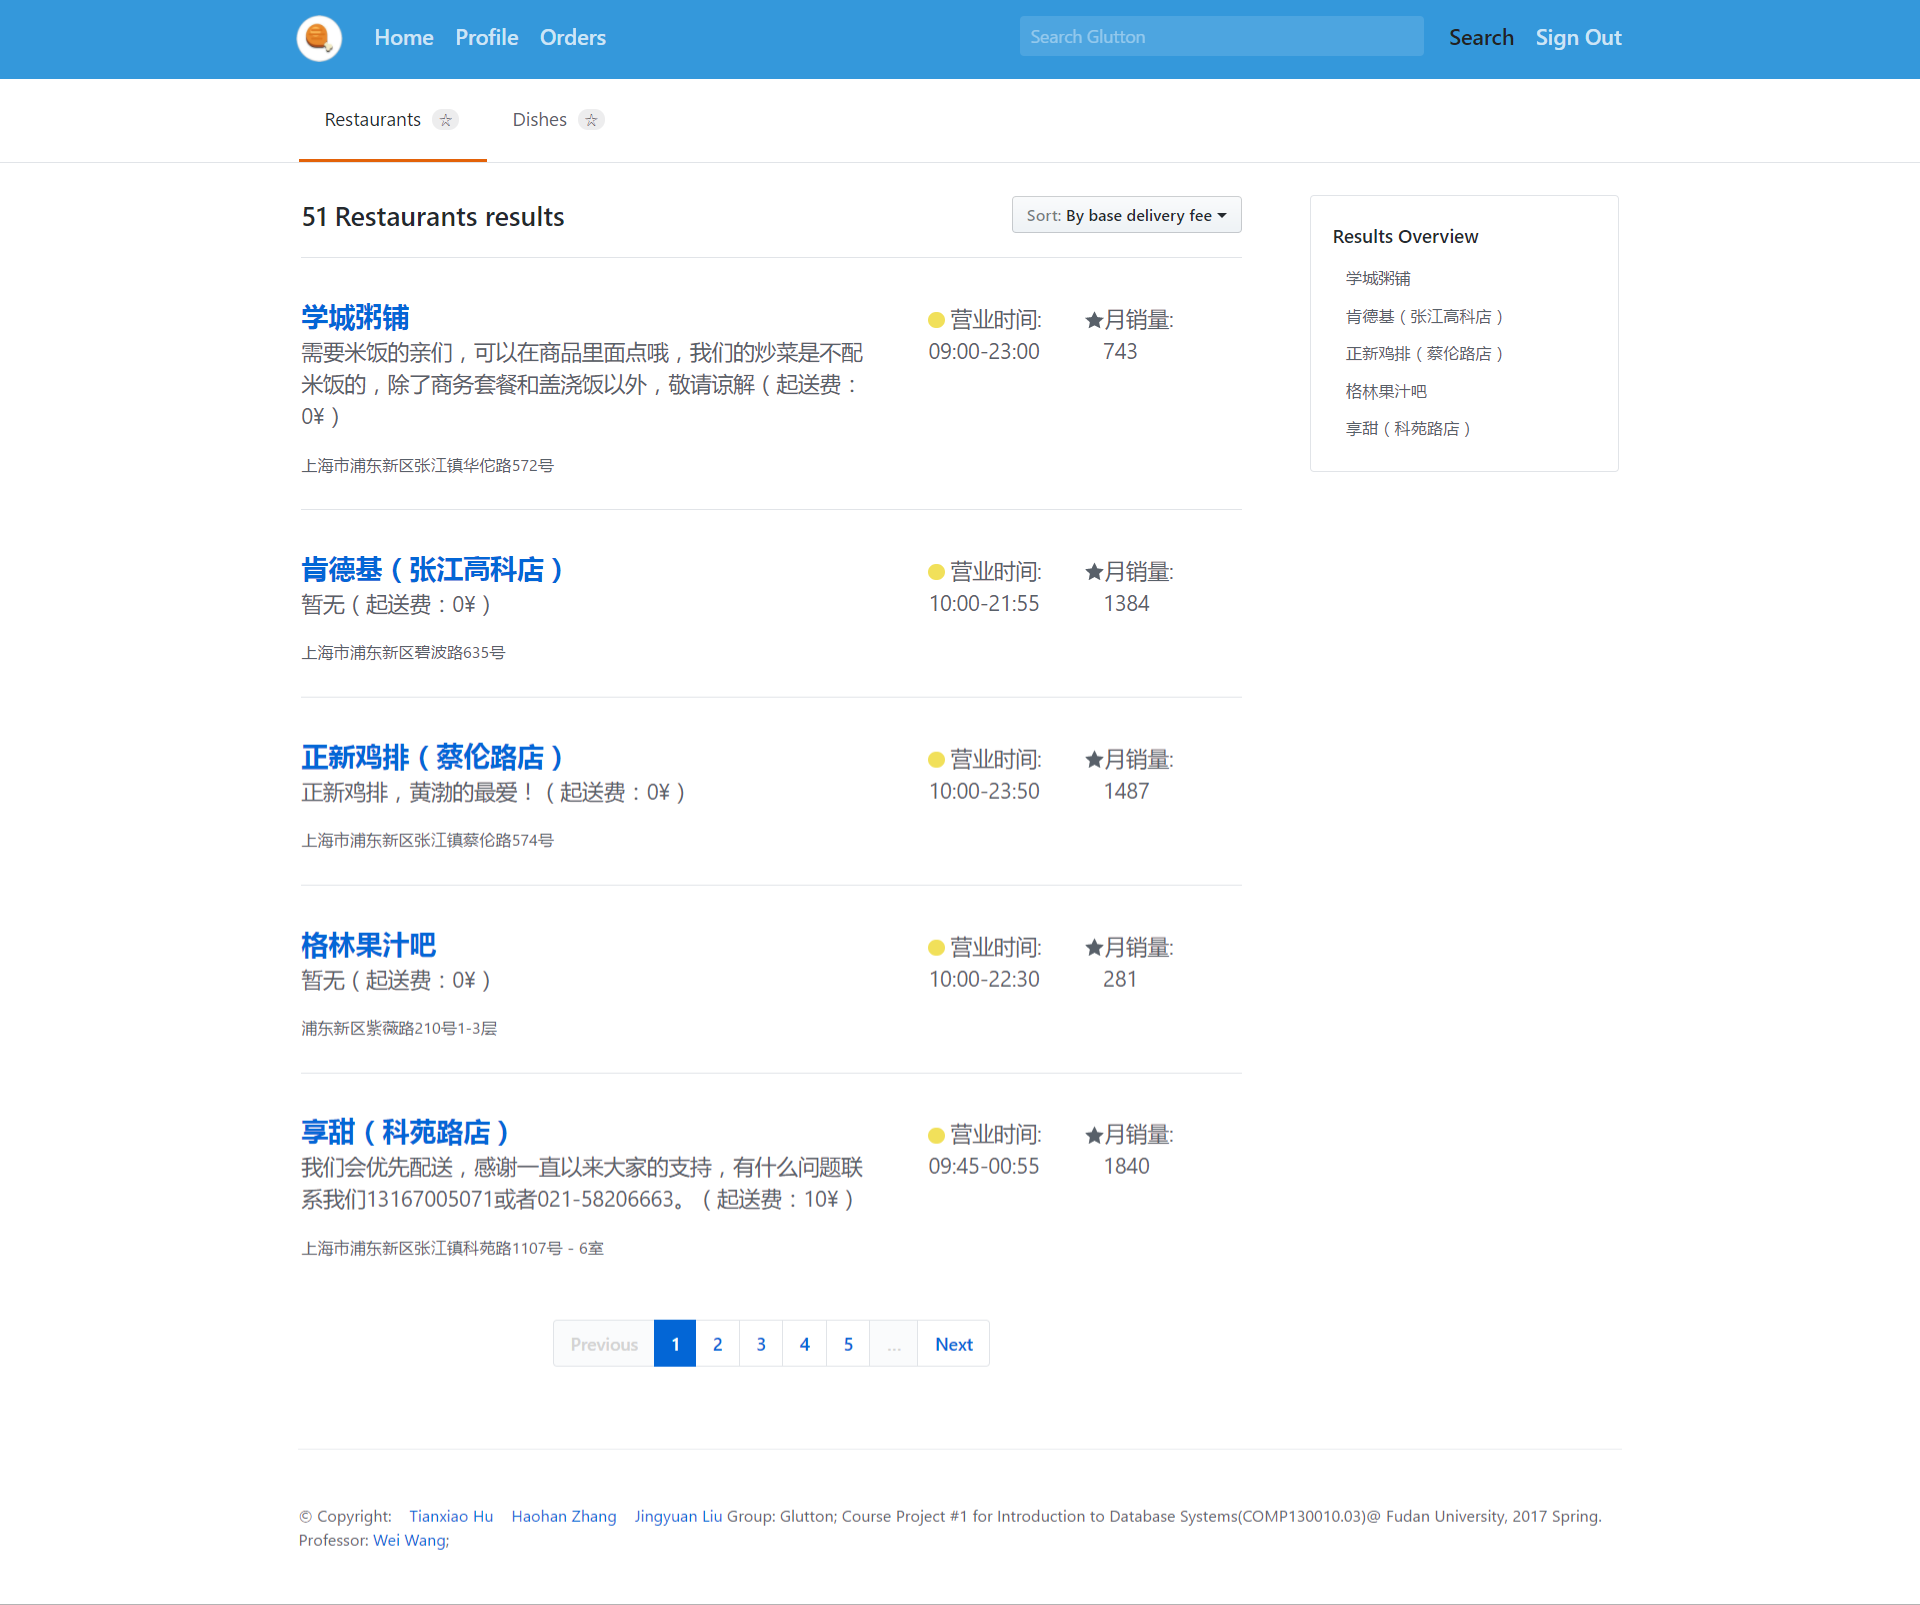
\includegraphics[width=6.00in]{cu-re.png}
     \caption{\small{用户查看商家列表}}
  \end{figure}
  \begin{figure}[H]
   \centering
     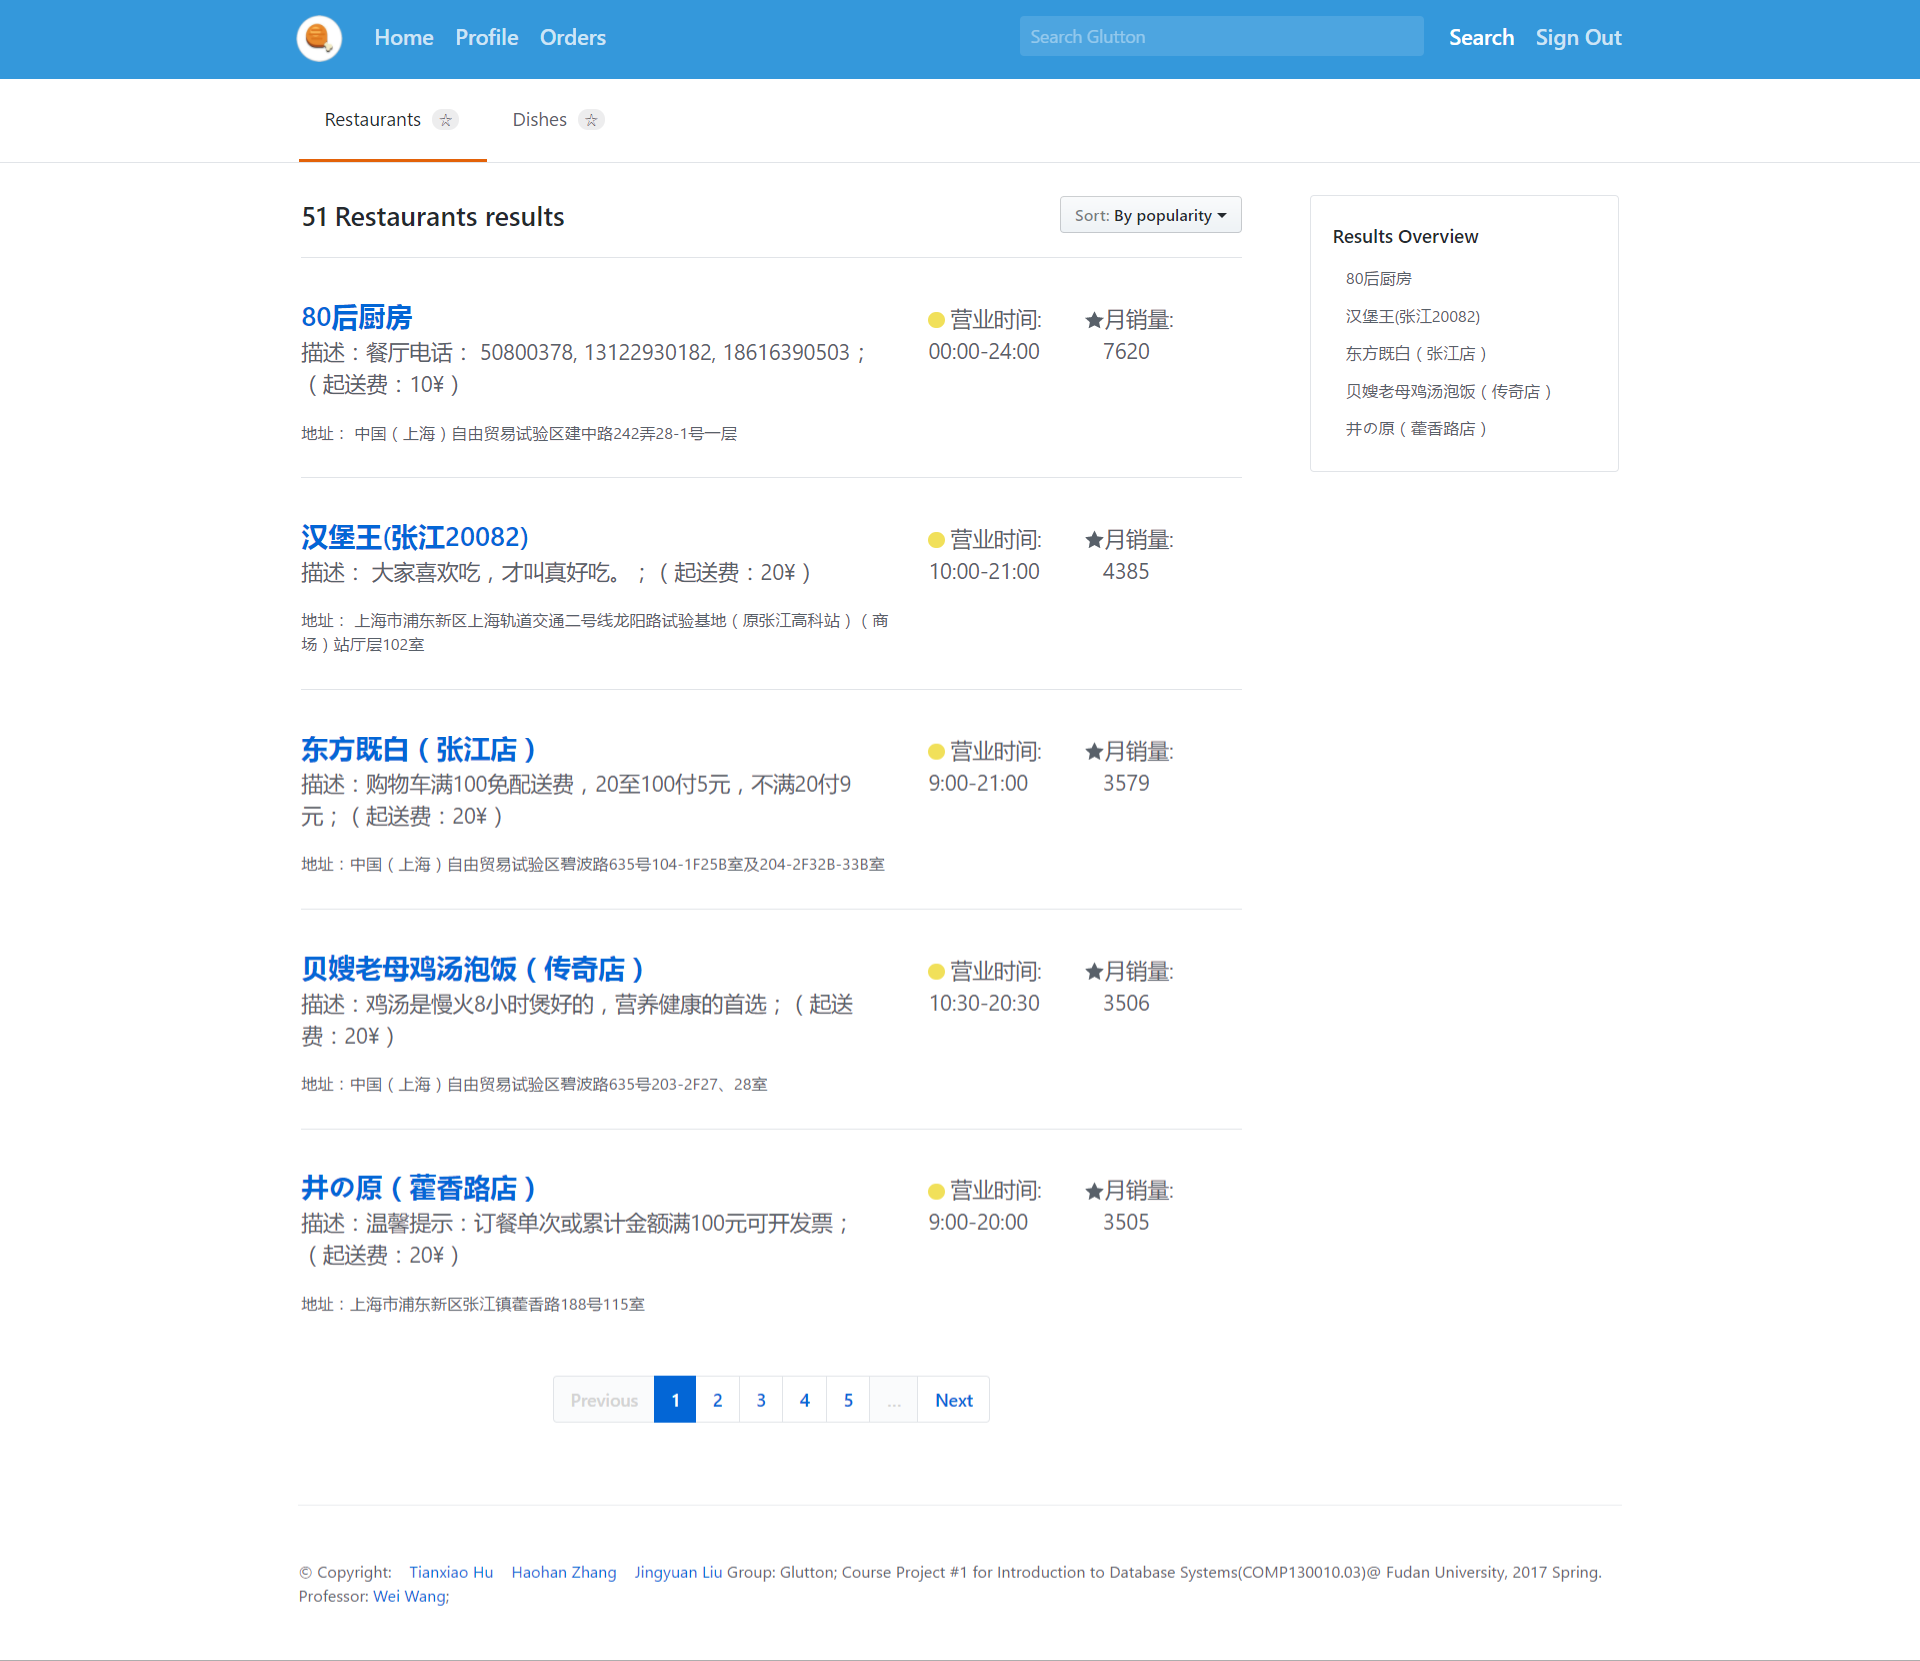
\includegraphics[width=6.00in]{cu-re-po.png}
     \caption{\small{用户按照月销量查看商家列表}}
  \end{figure}
  \item 下单\\
  跳转到商家页面,显示所有菜品,对每个菜品可以选择添加或删除,最后点击Submit Order提交订单。若用户已填写收货地址,则系统提示订单提交成功;若未填充,则选择继续并跳转到用户信息界面。
  \begin{figure}[H]
   \centering
     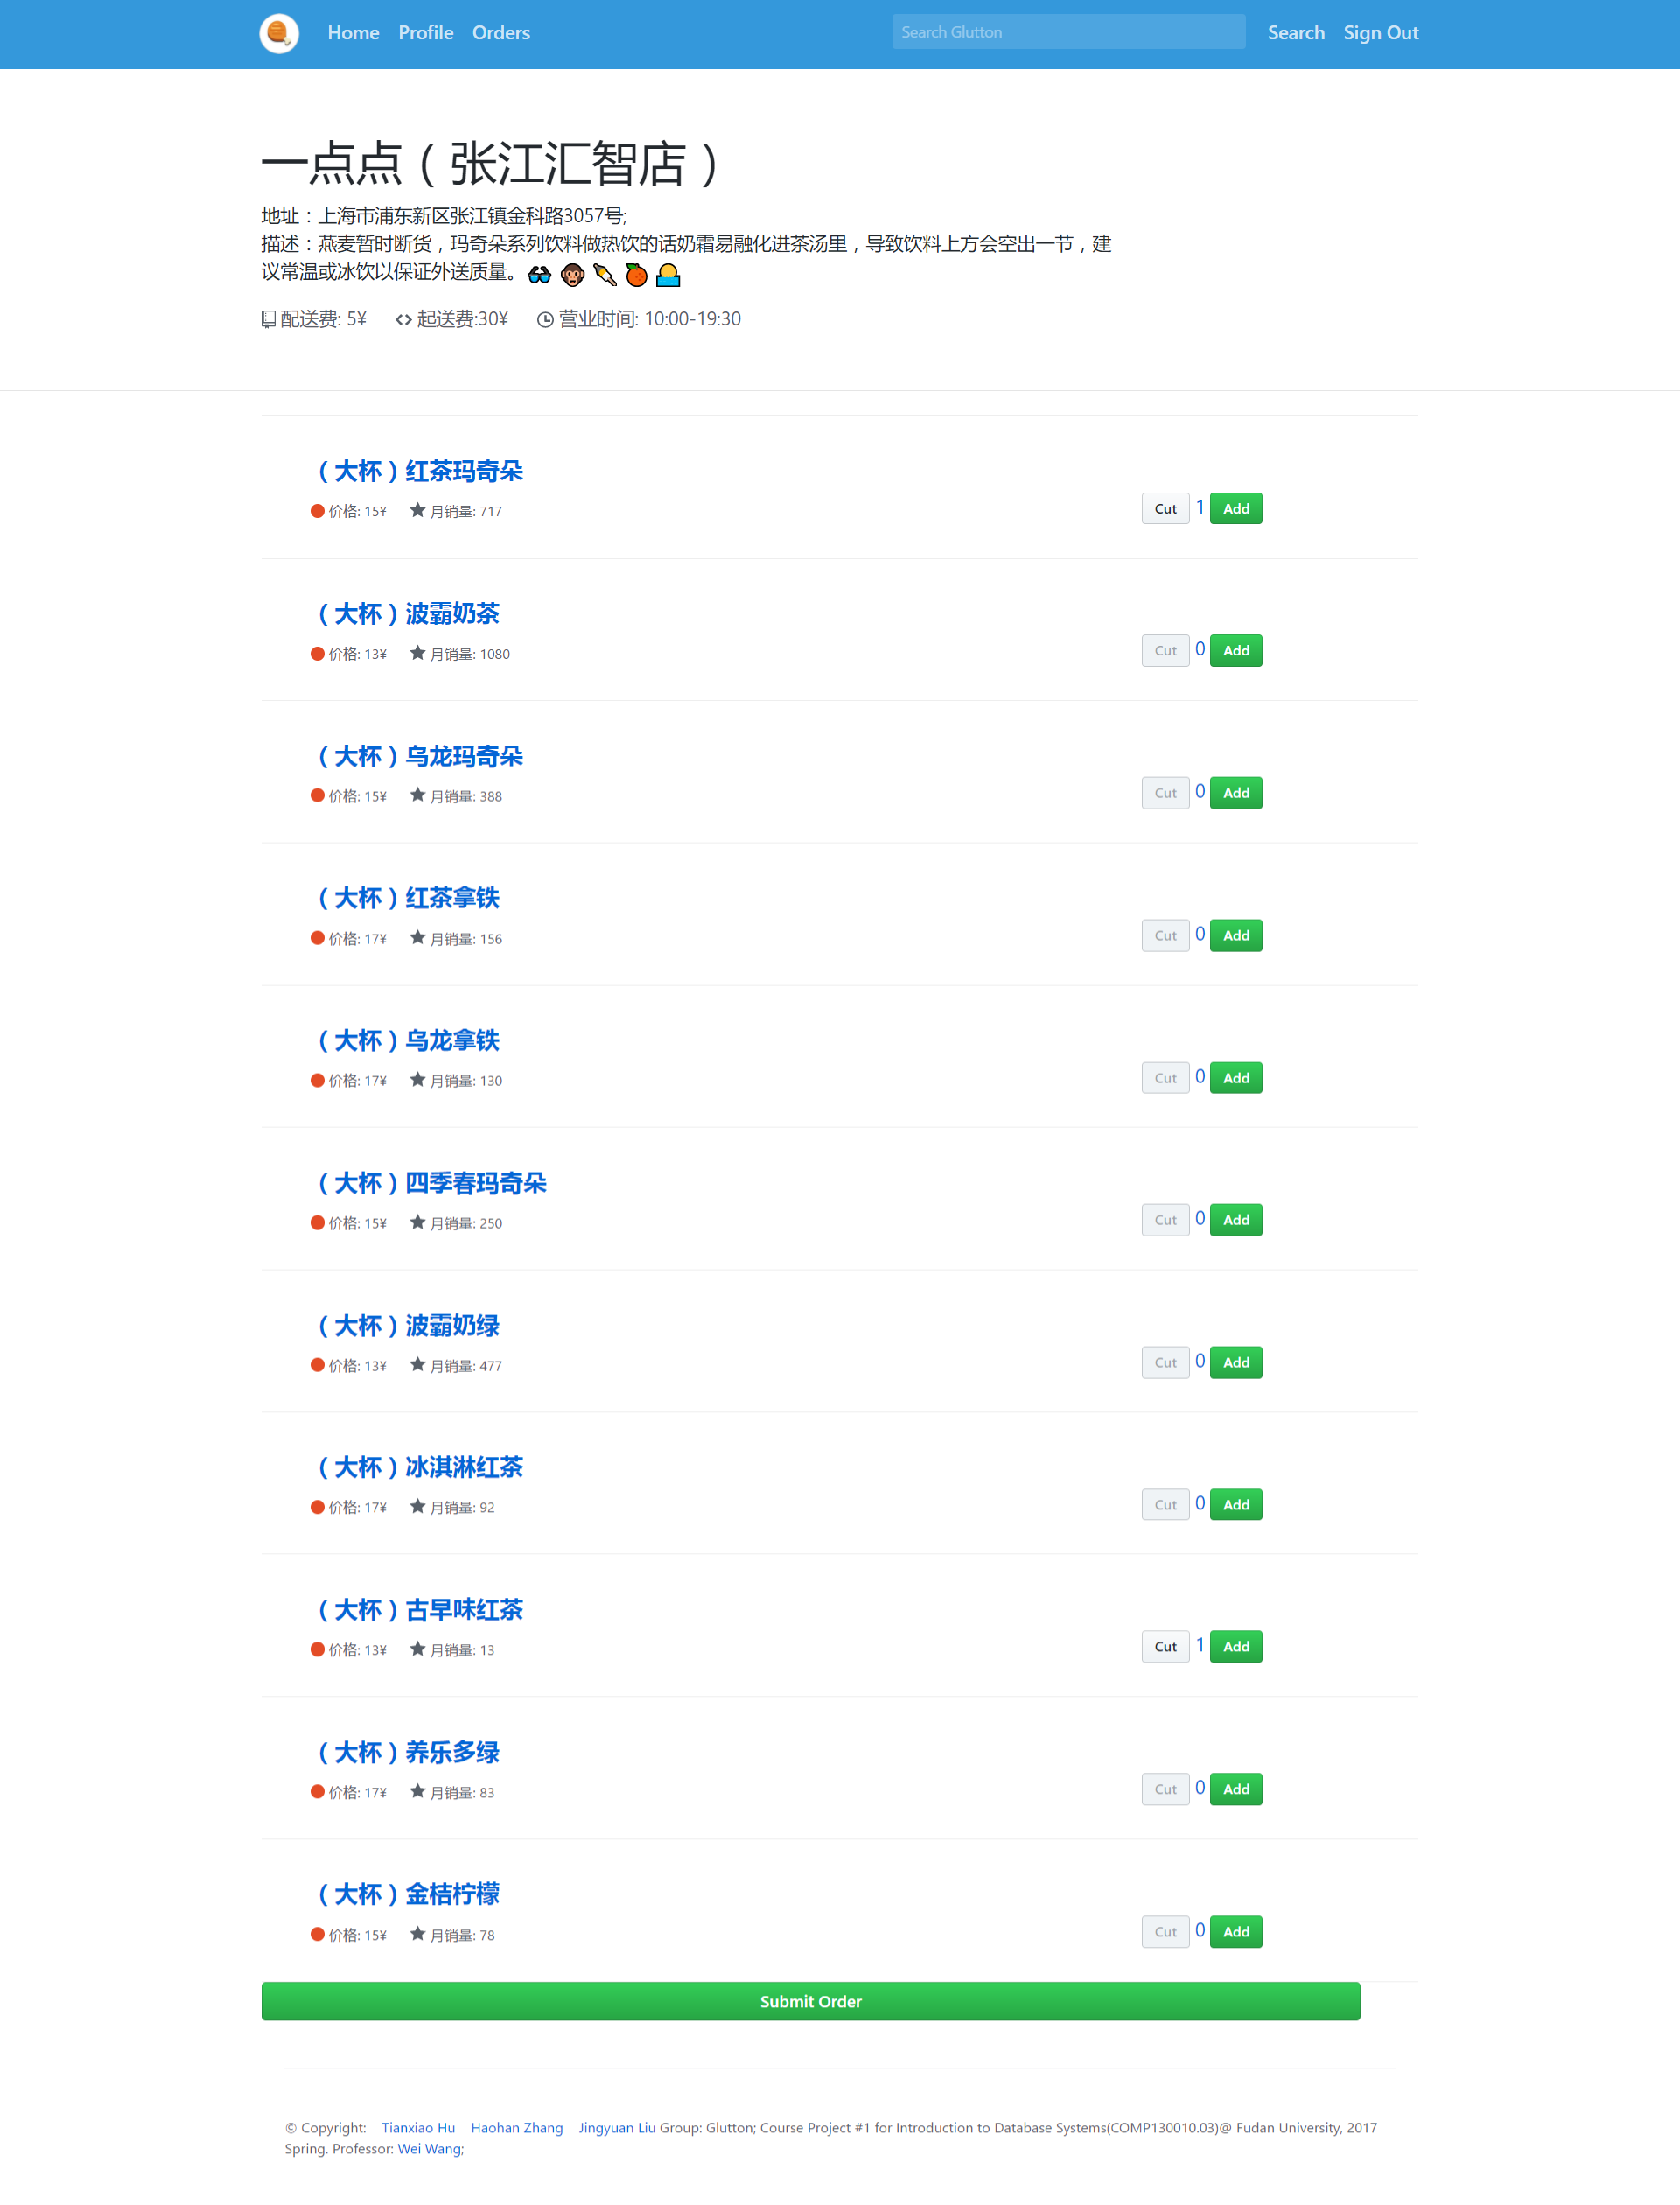
\includegraphics[width=6.00in]{cu-dish.png}
     \caption{\small{用户下单}}
  \end{figure}
  \begin{figure}[H]
   \centering
     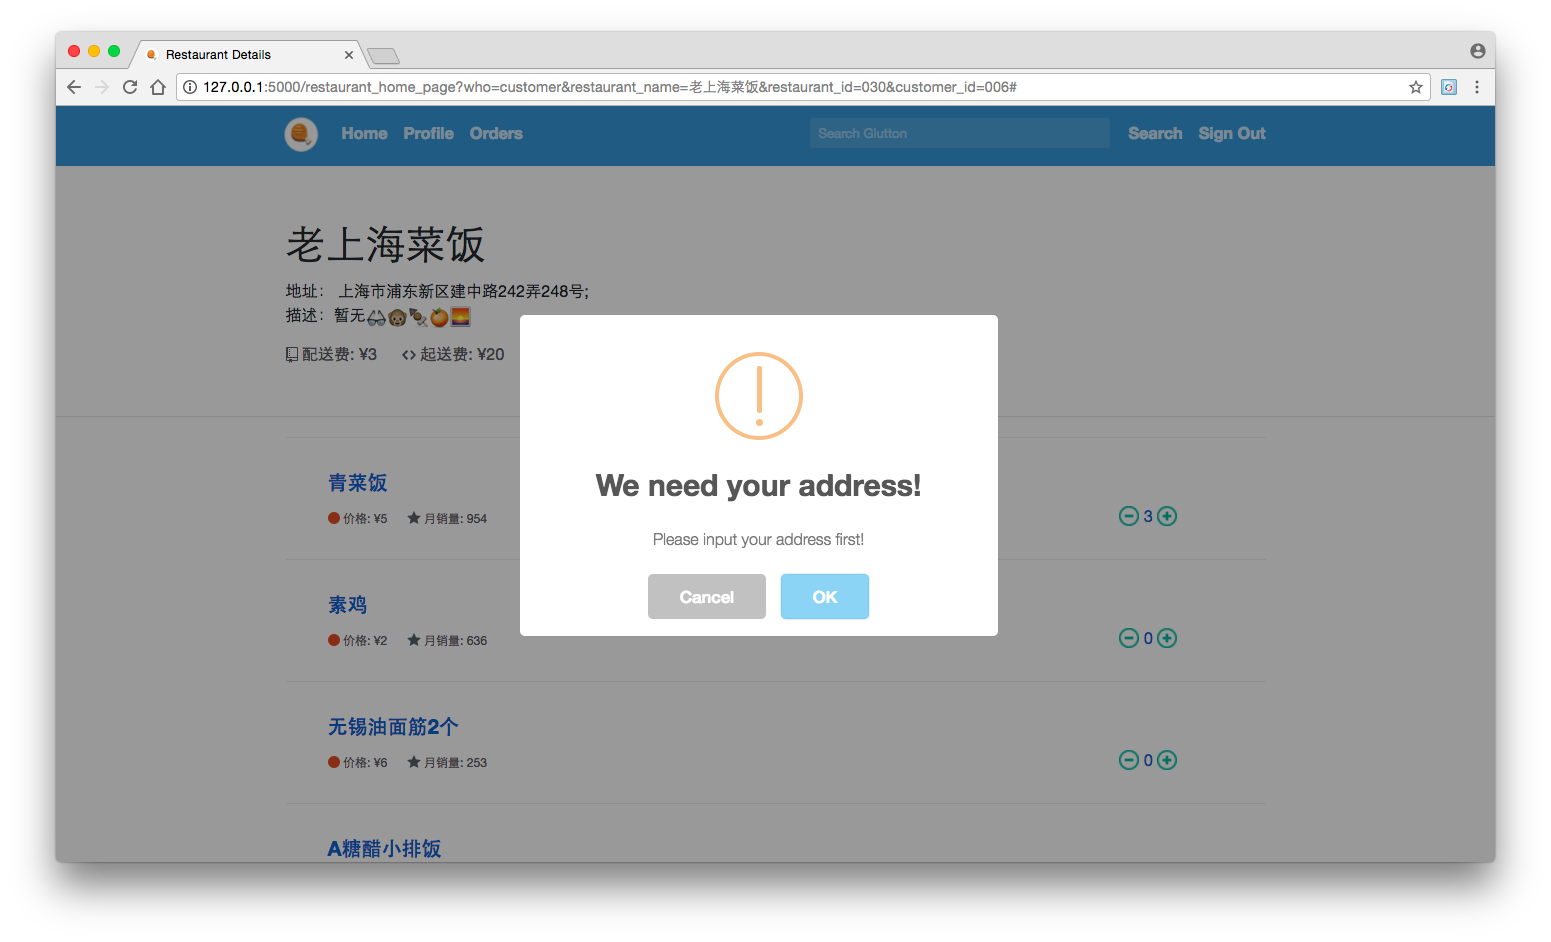
\includegraphics[width=6.00in]{cu-address.jpg}
     \caption{\small{用户未填充地址选择是否继续}}
  \end{figure}
  \item 收货\\
  点击order按钮,跳转到订单页面,可以查看所有订单信息。点击Received the Dishes确认收货。
  \begin{figure}[H]
   \centering
     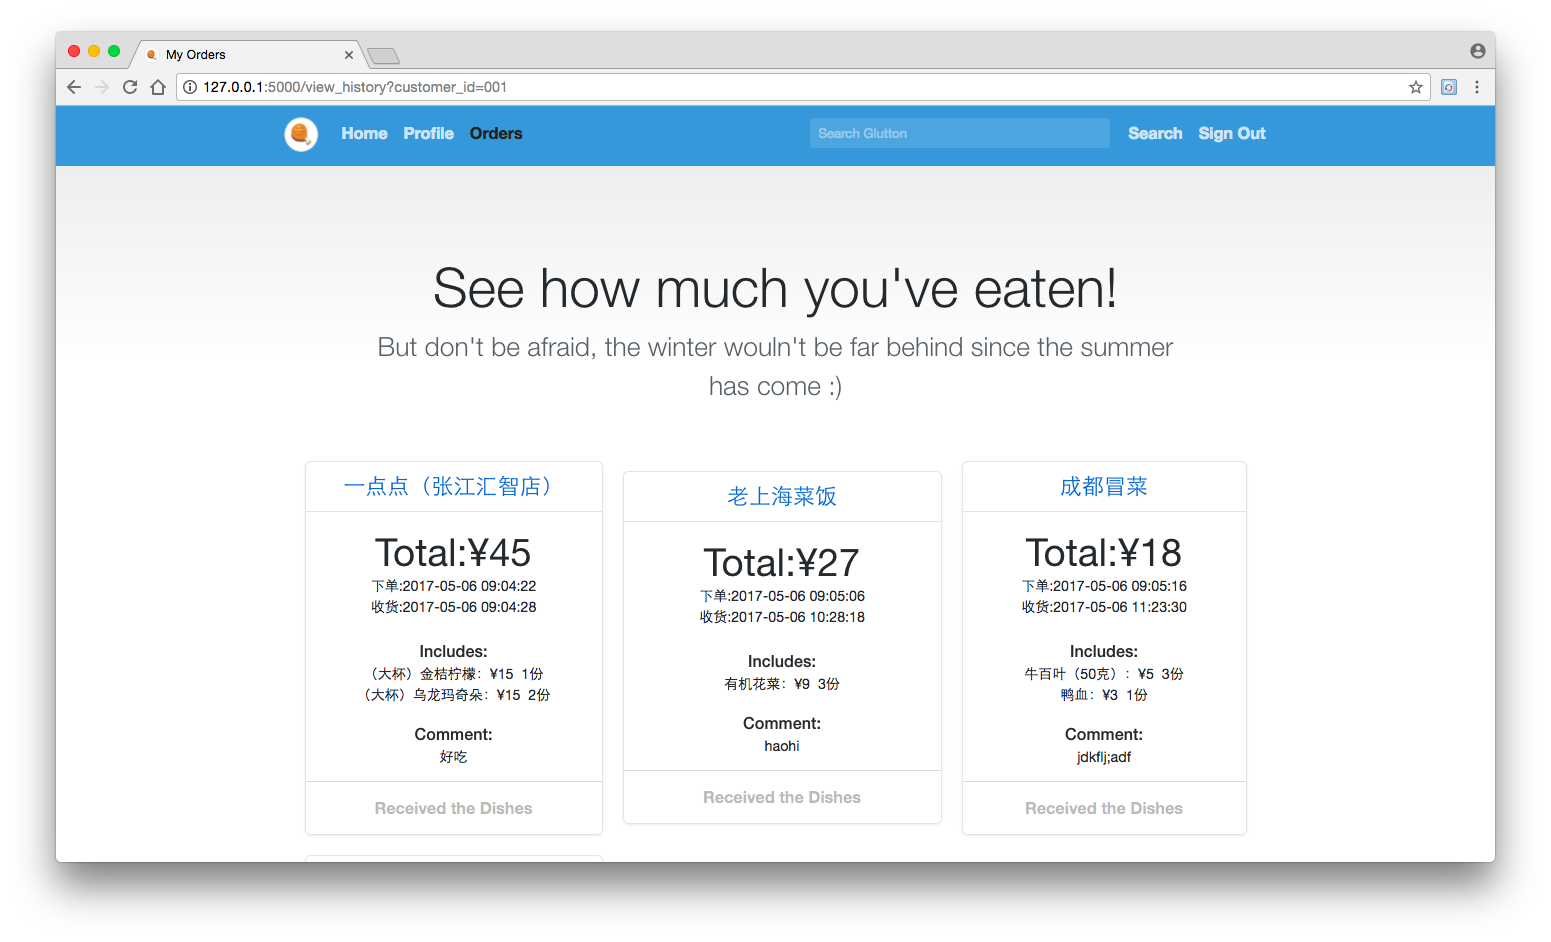
\includegraphics[width=6.00in]{cu-order.jpg}
     \caption{\small{用户查看订单确认收货}}
  \end{figure}
  \item 评论\\
  点击确认收货按钮后,会弹出评价窗口,用户可以写评价,系统提示提交评价成功,跳转到订单界面。
  \begin{figure}[H]
   \centering
     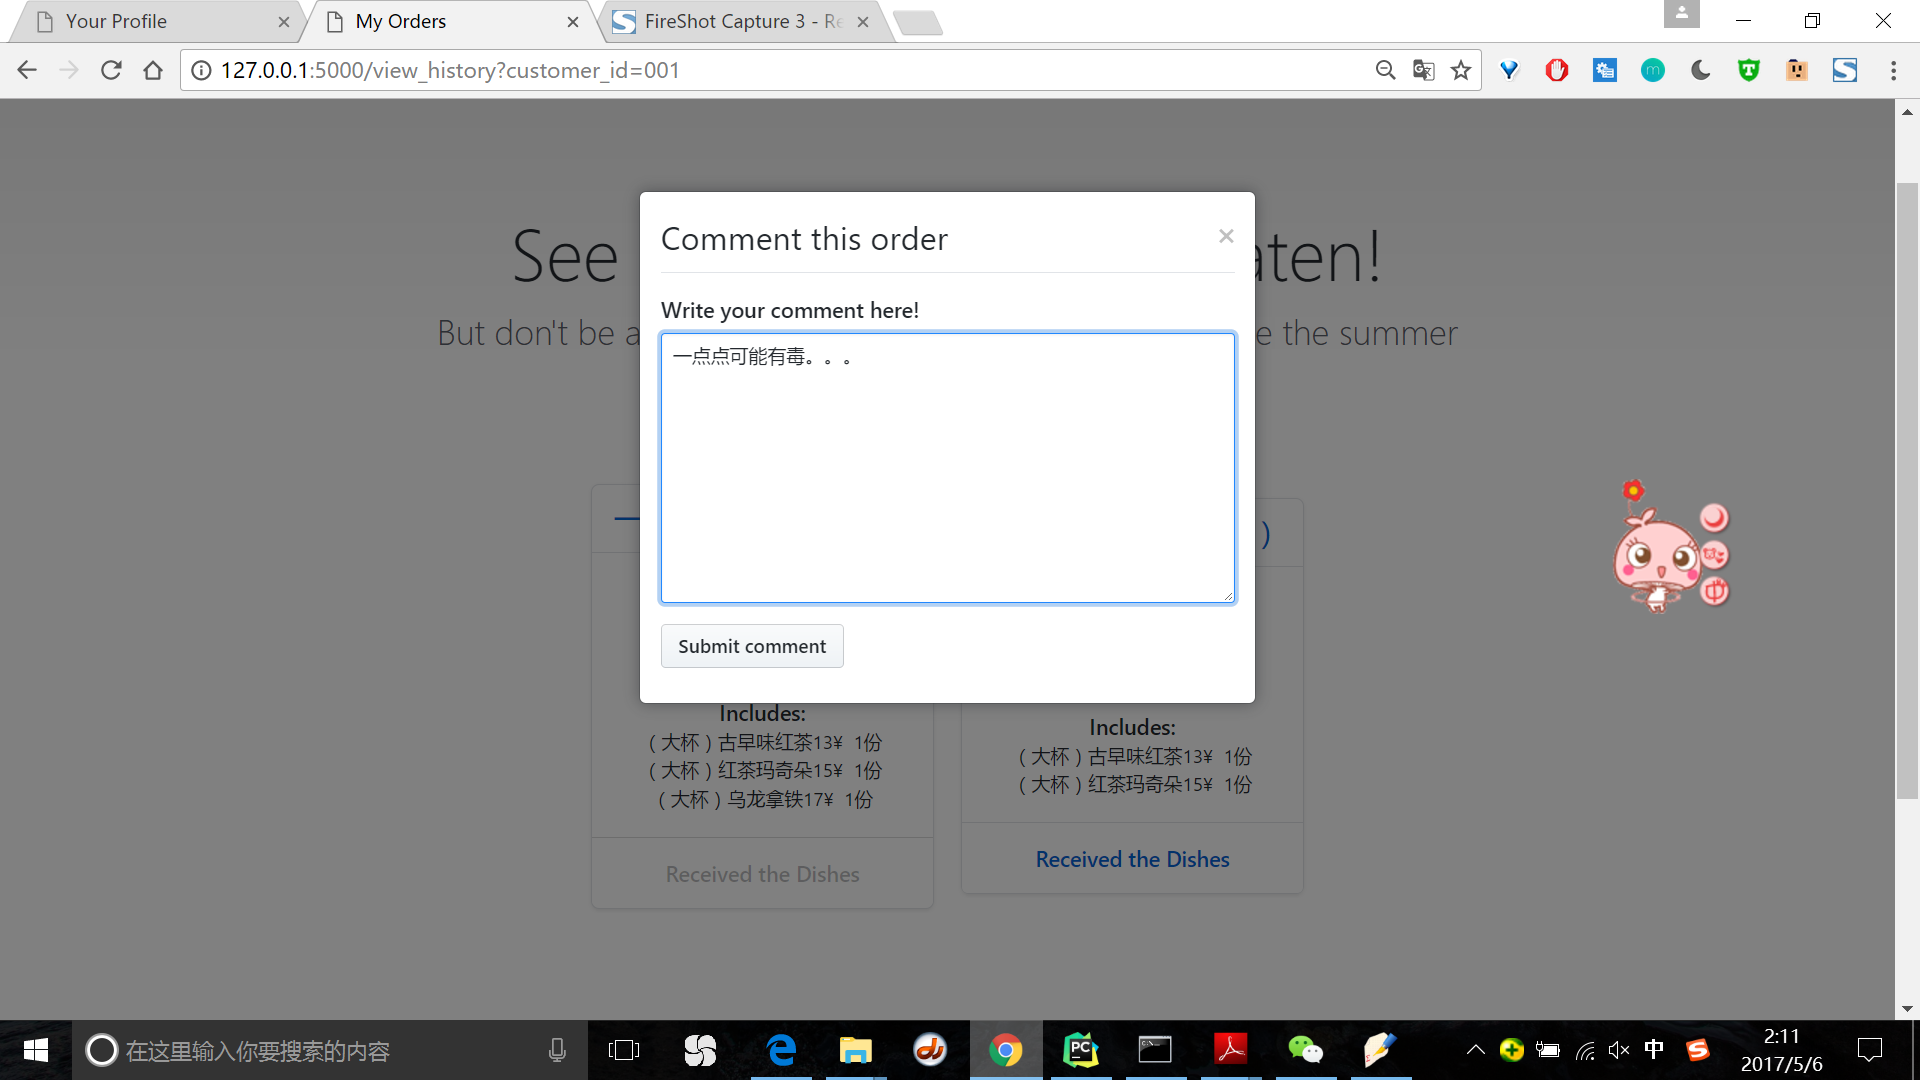
\includegraphics[width=5.50in]{cu-comment.jpg}
     \caption{\small{用户填写评价}}
  \end{figure}
  \end{itemize}

 \subsection{针对商家的功能}
 商家主界面与用户类似,右侧和中部为登录商家和注册商家按钮。
 \begin{figure}[H]
   \centering
     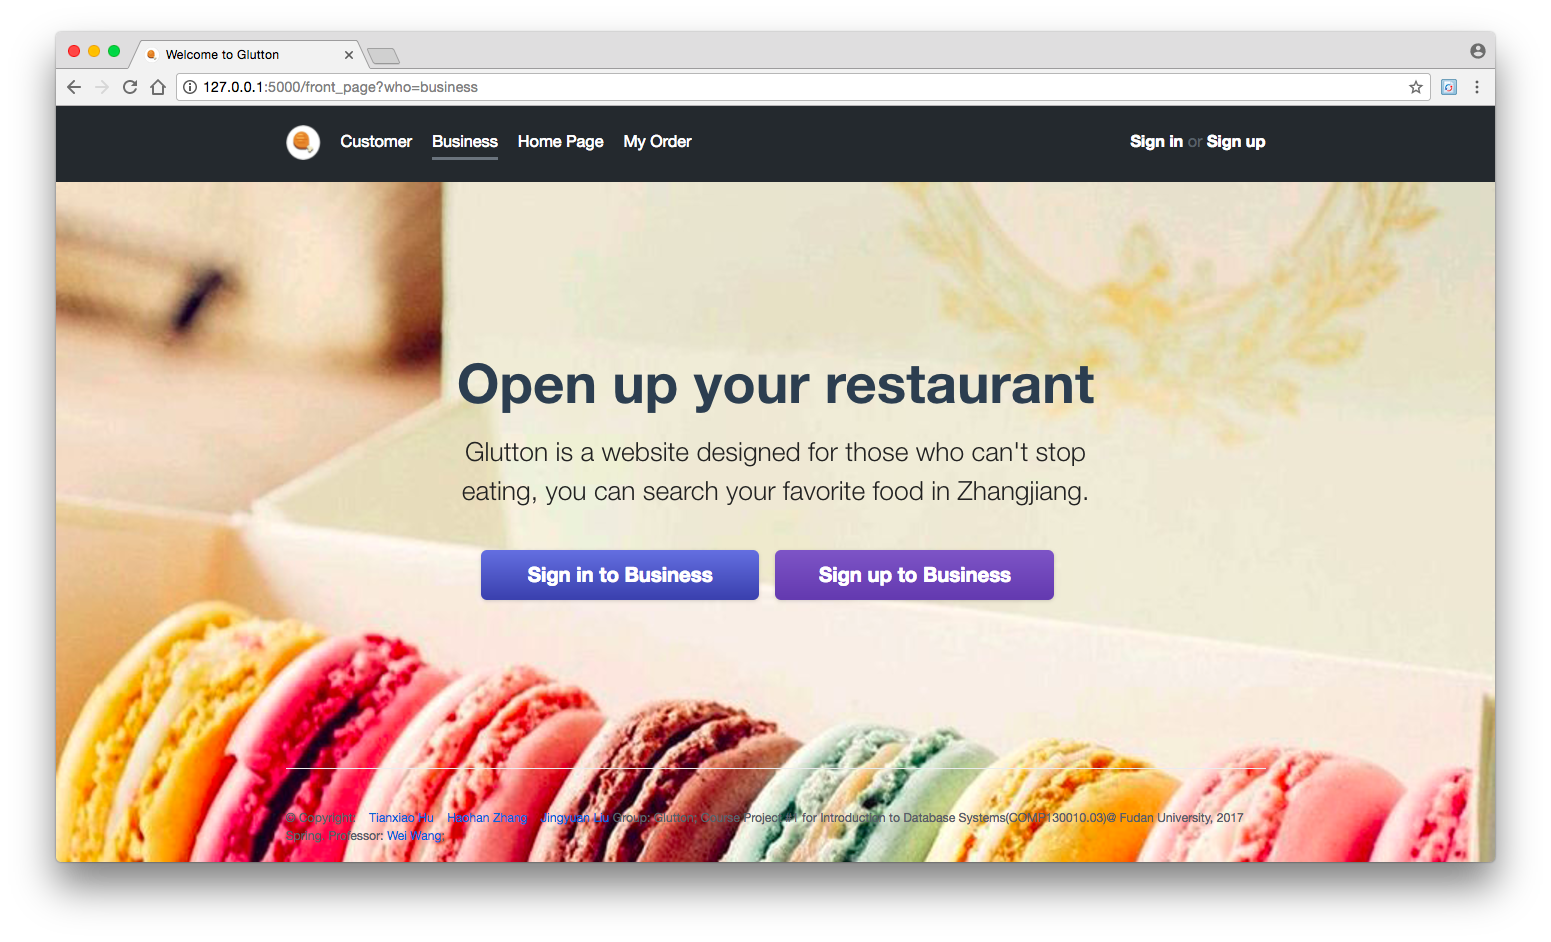
\includegraphics[width=5.80in]{re-front.png}
     \caption{\small{主页面}}
  \end{figure}
  \begin{itemize}
  \item 注册/登录\\
  点击sign up to business按钮我们进入商家注册页面,输入用户名,店铺名,密码来注册。\\
  点击sign in to business按钮我们进入商家登录页面,用用户名和密码登录。如果用户名输入错误,系统会提示商家不存在;如果密码输入错误,系统会提示密码错误。
  \begin{figure}[H]
   \begin{minipage}[t]{0.5\linewidth}
    \centering
     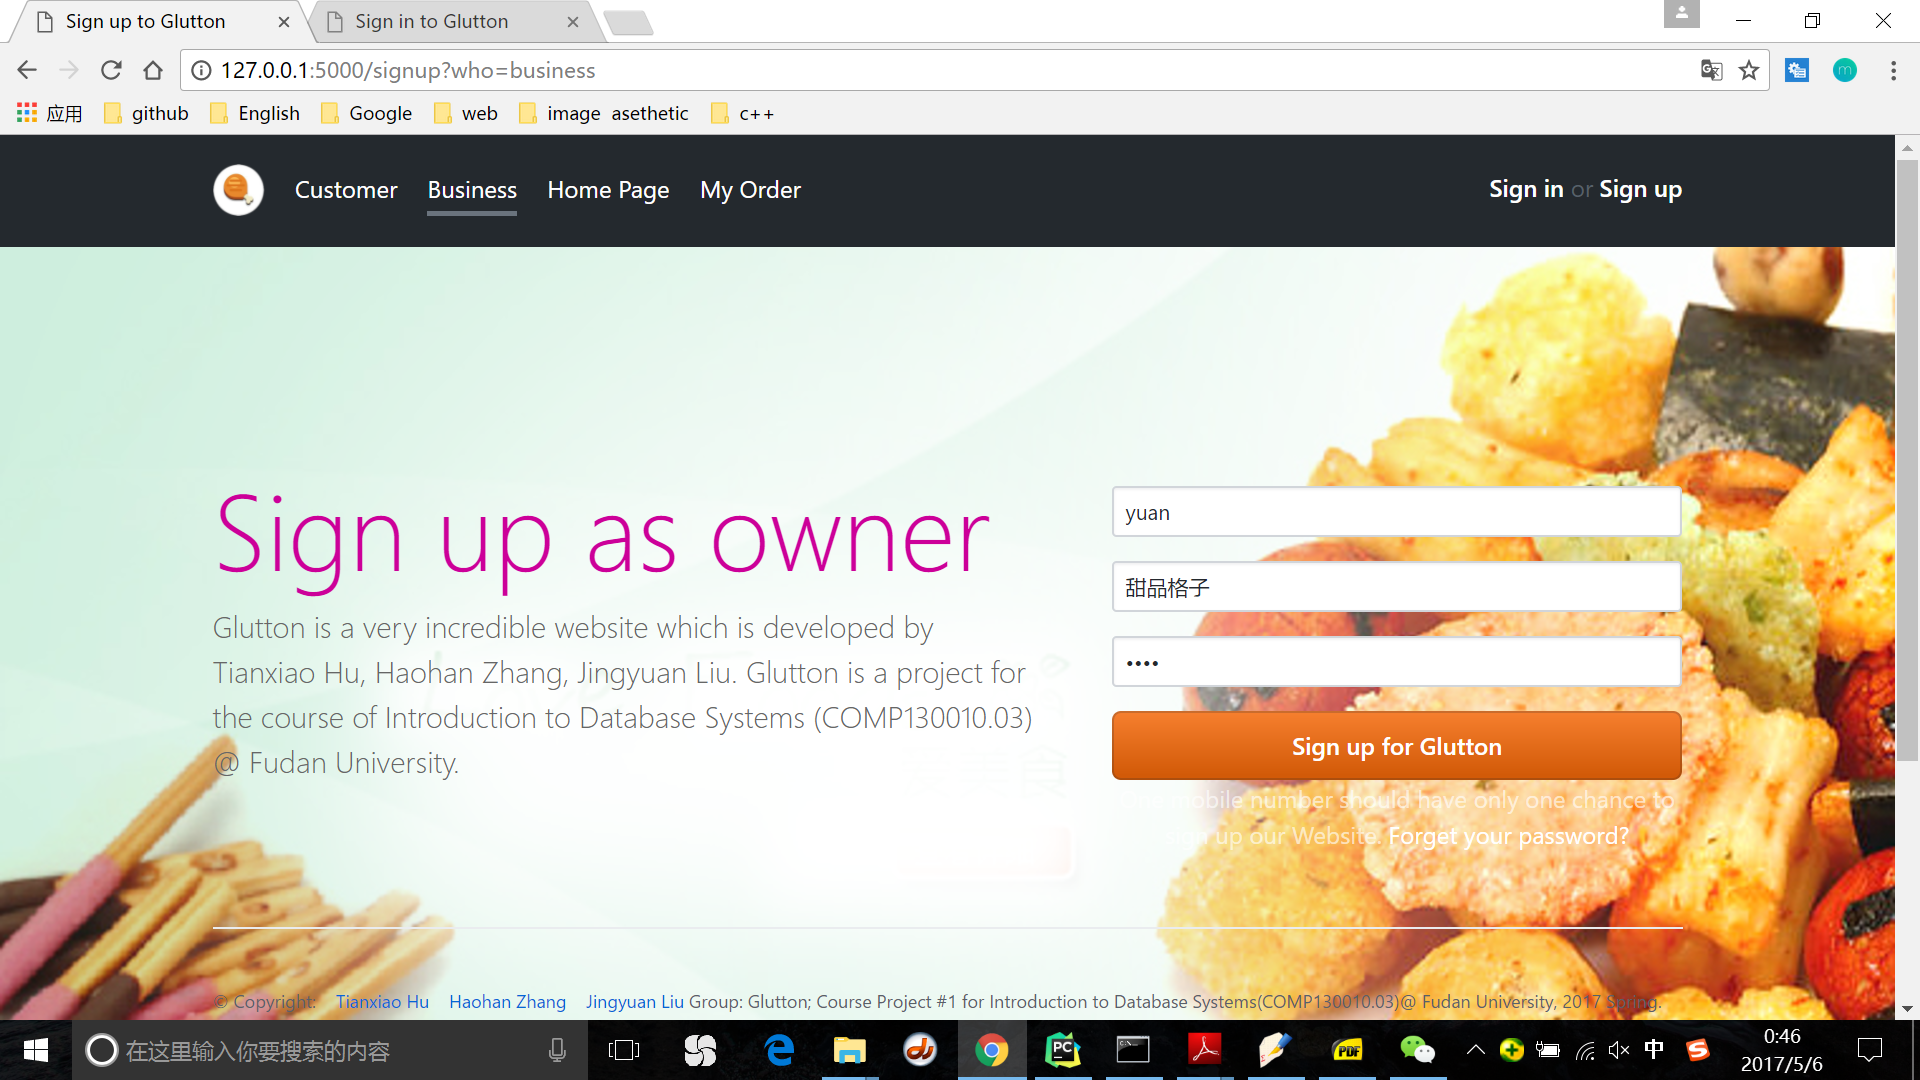
\includegraphics[width=3.2in]{re-signup.jpg}
     \caption{\small{商家注册}}
   \end{minipage}
   \begin{minipage}[t]{0.5\linewidth}
    \centering
     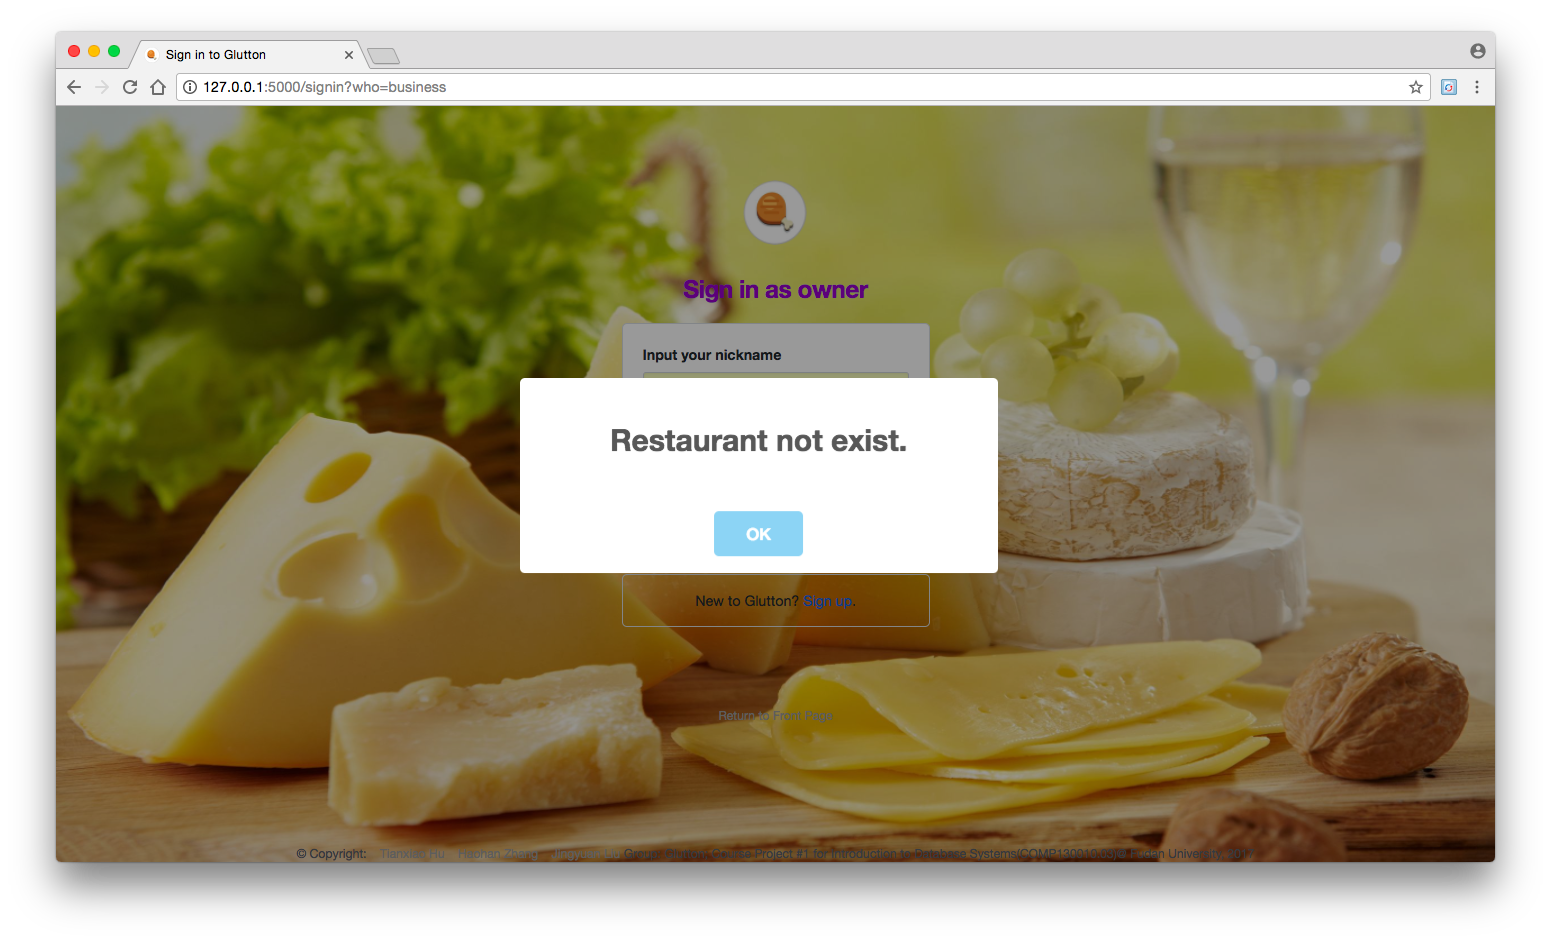
\includegraphics[width=3.2in]{re-signin.jpg}
      \caption{\small{商家登录并显示该商家不存在}}
   \end{minipage}
   \end{figure}
  \item 更改信息\\
  登录成功后,我们进入到商家的主页。主页的最上方是导航栏,左侧四个按钮可以选择主页,商家信息,菜品,订单。右侧有搜索栏和退出登录按钮。\\
  左侧显示用户名和商家号,及修改商家信息按钮。
  \begin{figure}[H]
   \centering
     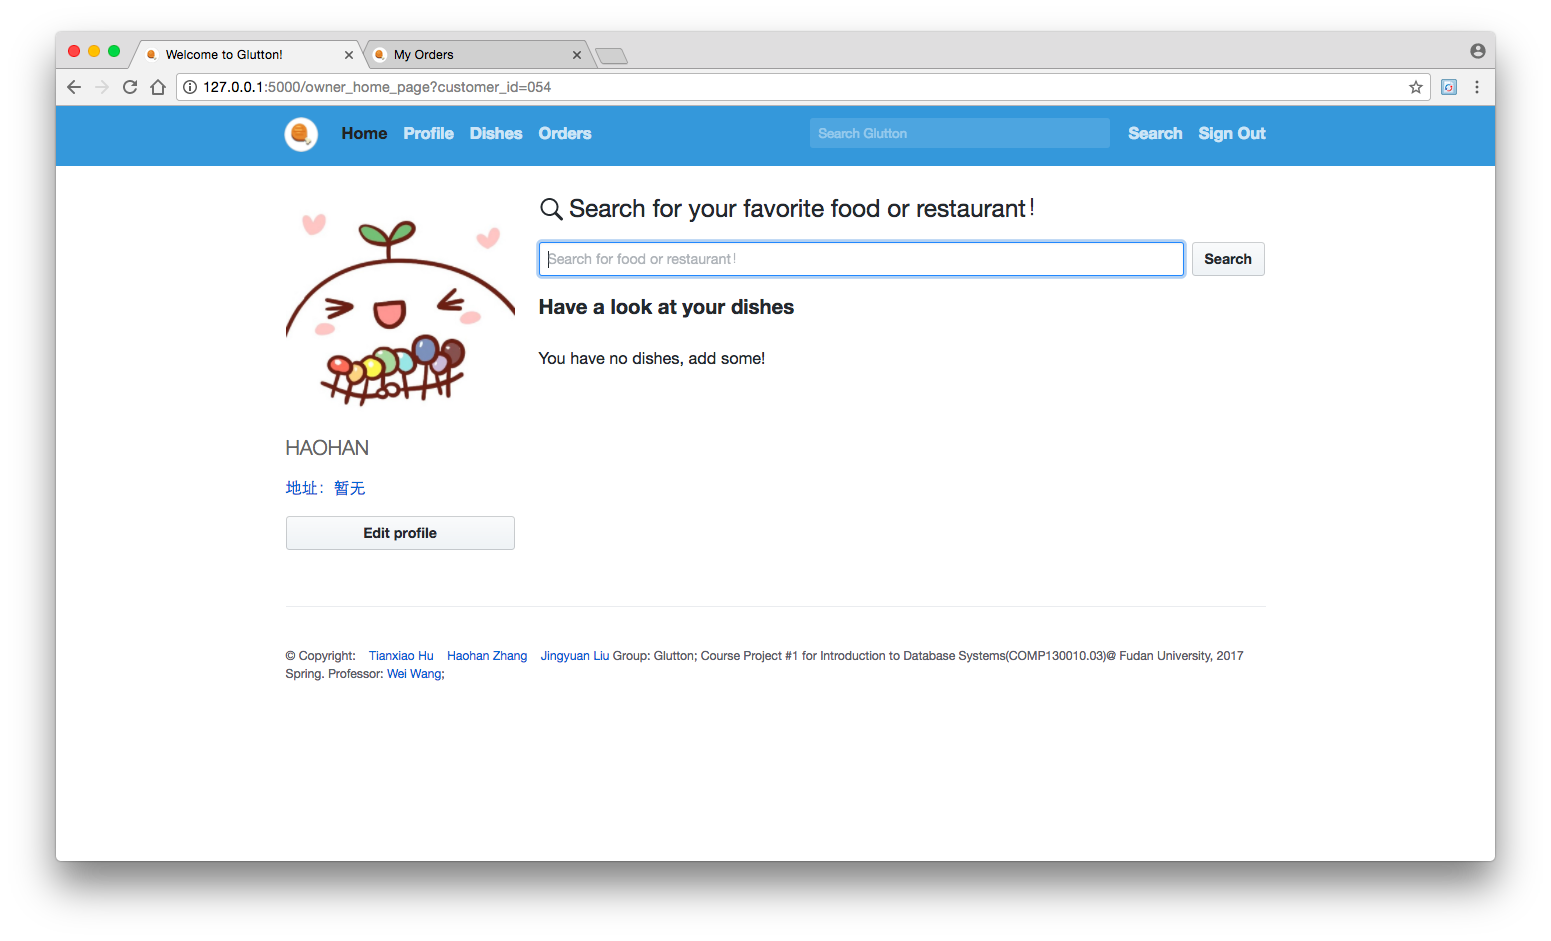
\includegraphics[width=6.00in]{re-home1.jpg}
     \caption{\small{商家主页(无菜品时)}}
  \end{figure}
  \begin{figure}[H]
   \centering
     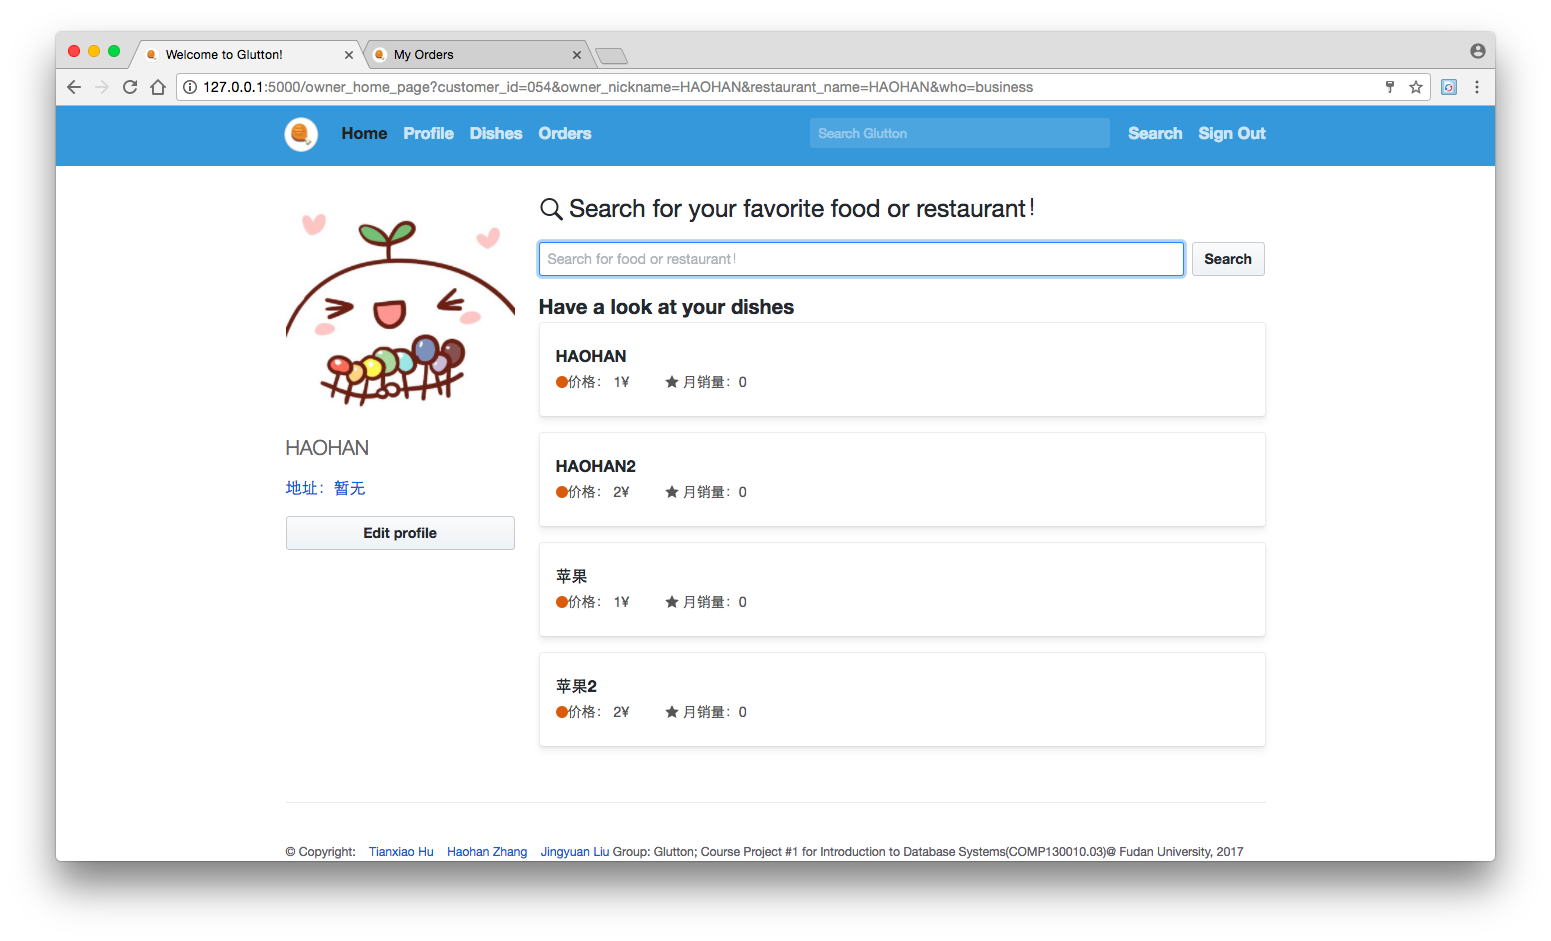
\includegraphics[width=6.00in]{re-home2.jpg}
     \caption{\small{商家主页(有菜品时)}}
  \end{figure}
  点击Edit profile按钮进入修改商家信息页面,左侧可以选择类型:基本信息,更改密码,查看订单,管理菜品,添加菜品,退出登录。\\
  基本信息可以修改店铺名、地址、配送费、起送价、平均配送时间和店铺公告;密码修改,如果修改成功,系统会提示“Succeed”
  \begin{figure}[H]
   \begin{minipage}[t]{0.5\linewidth}
    \centering
     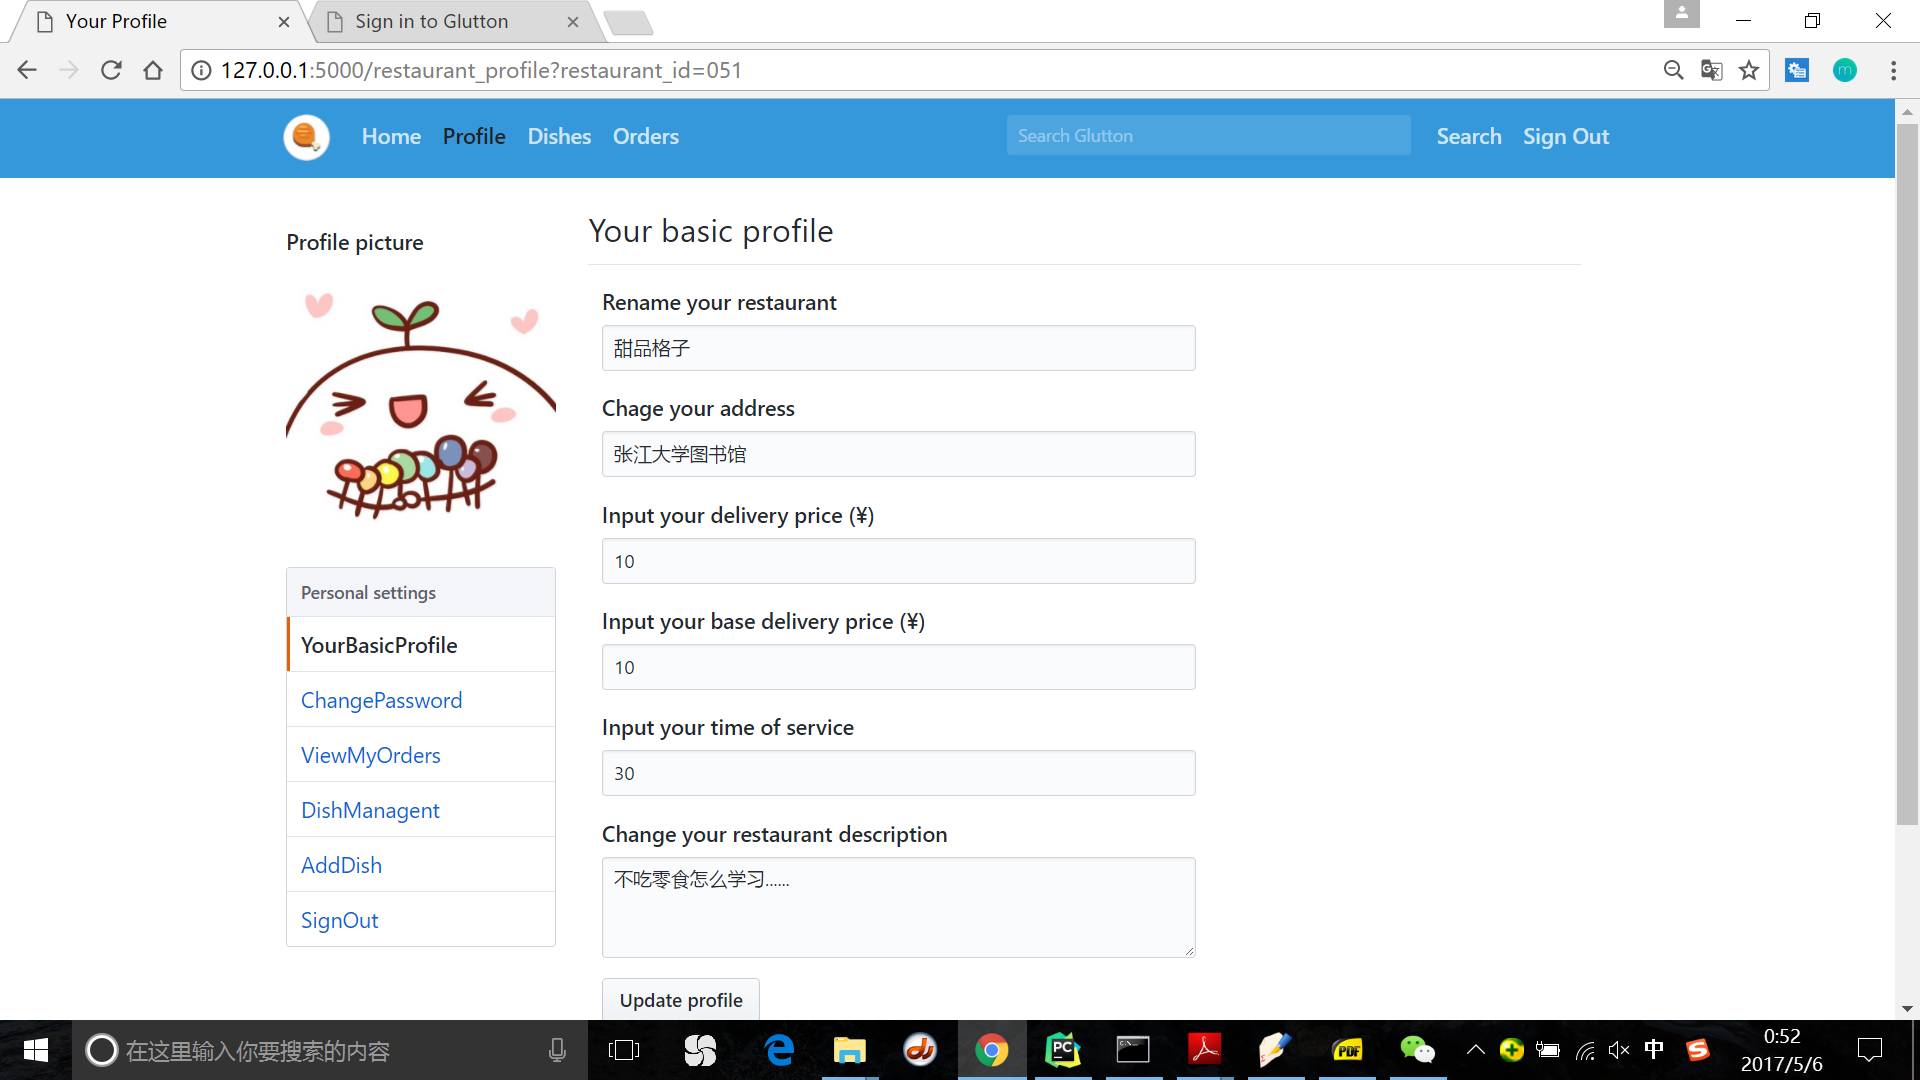
\includegraphics[width=3.2in]{re-profile.jpg}
     \caption{\small{商家更改信息}}
   \end{minipage}
   \begin{minipage}[t]{0.5\linewidth}
    \centering
     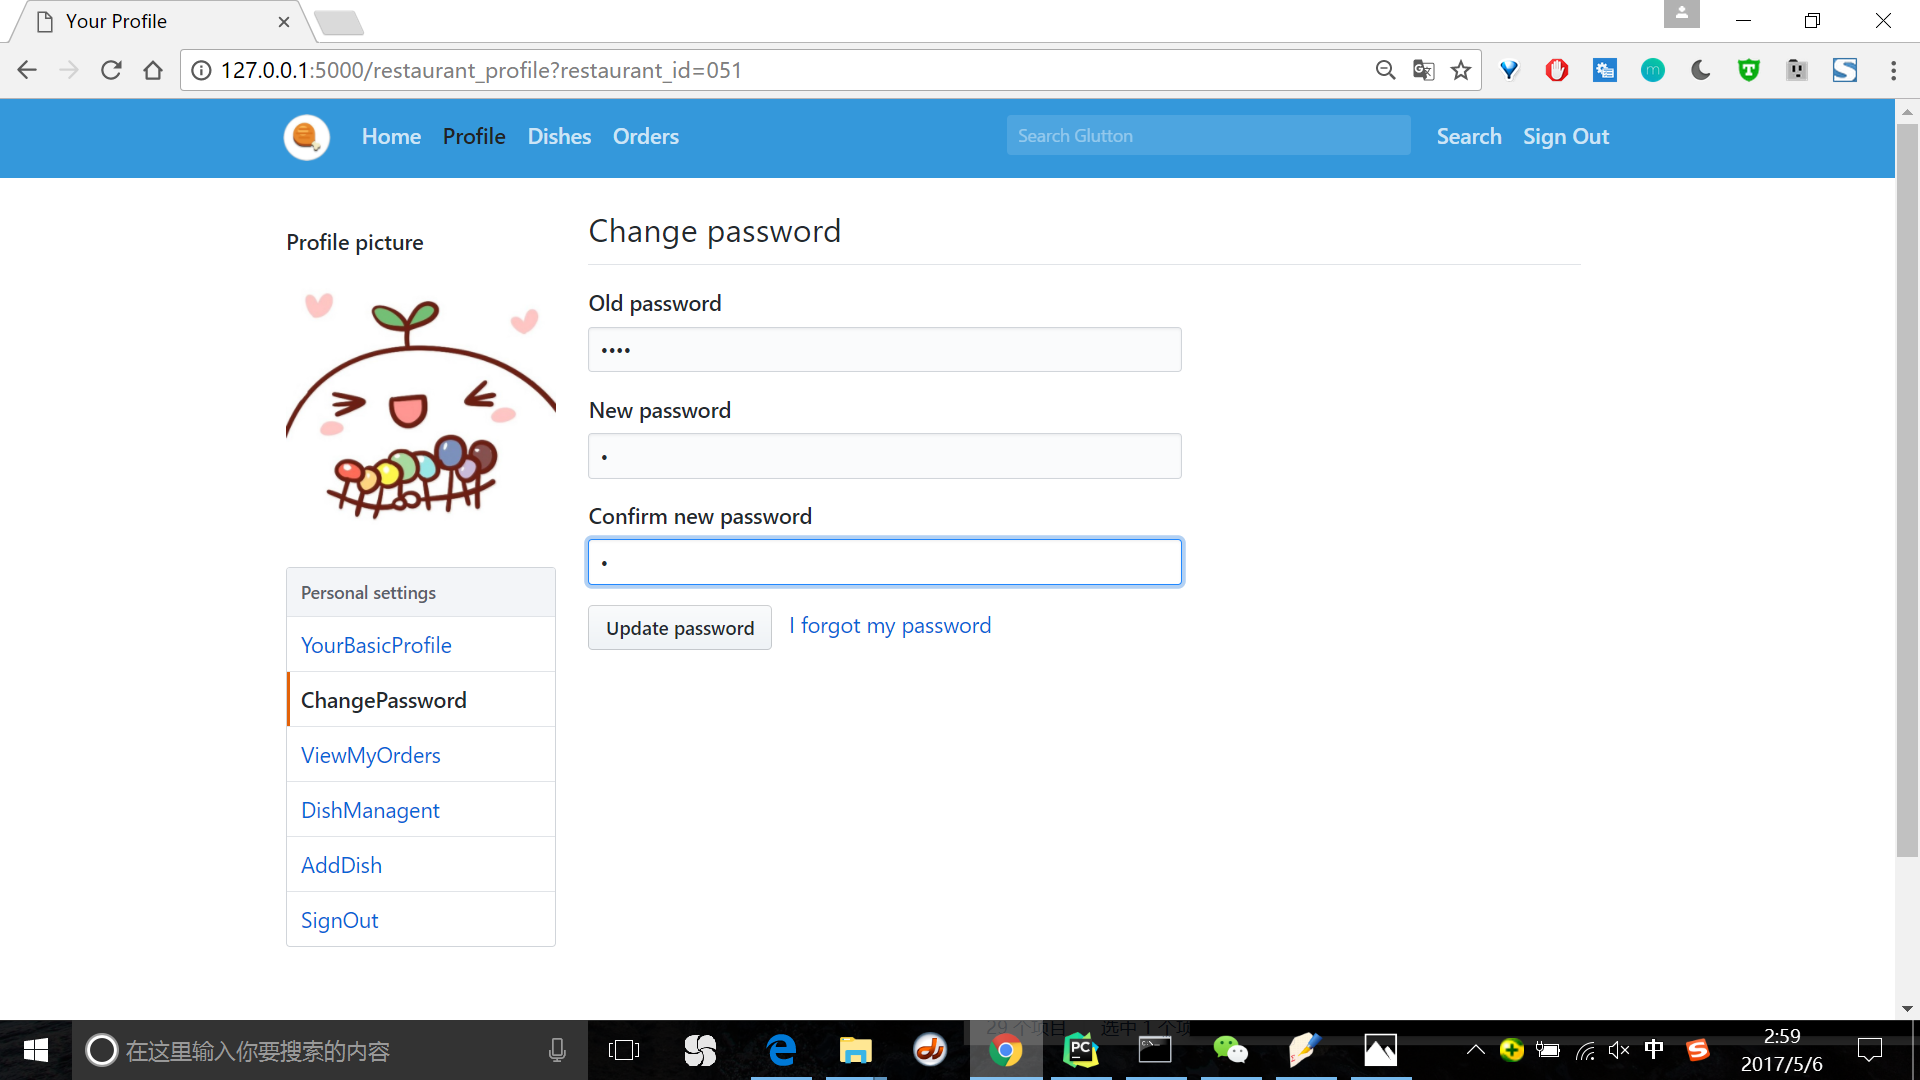
\includegraphics[width=3.2in]{re-password.jpg}
      \caption{\small{商家更改密码}}
   \end{minipage}
   \end{figure}
  \item 增加菜品\\
  点击AddDish按钮可以添加菜品,需要填写菜品名和价格,菜品添加成功,系统提示载入成功。\\
  我们也可以点击左侧DishManagement,或导航栏的Dishes进入菜品管理页面,会显示已有的菜品,并可以执行编辑、增加、删除操作。
  \begin{figure}[H]
   \begin{minipage}[t]{0.5\linewidth}
    \centering
     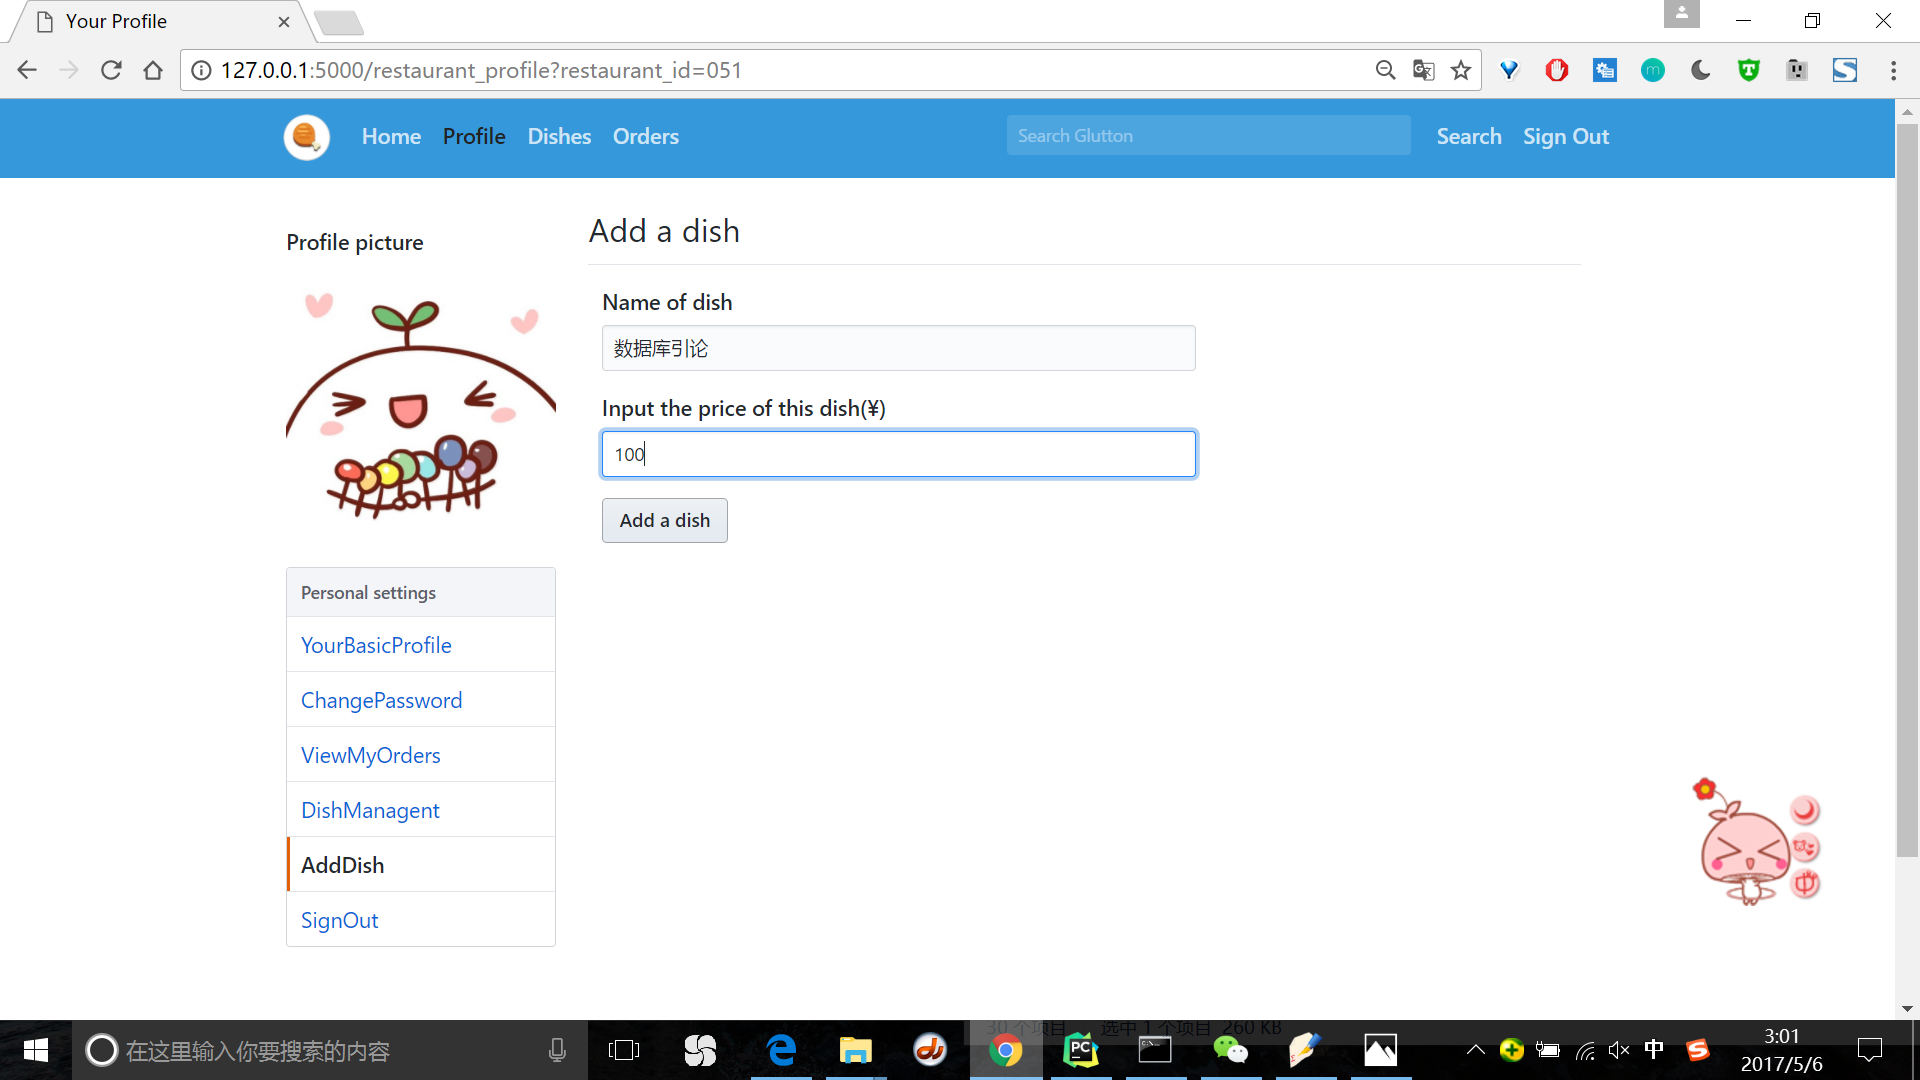
\includegraphics[width=3.2in]{re-add.jpg}
     \caption{\small{商家增加菜品}}
   \end{minipage}
   \begin{minipage}[t]{0.5\linewidth}
    \centering
     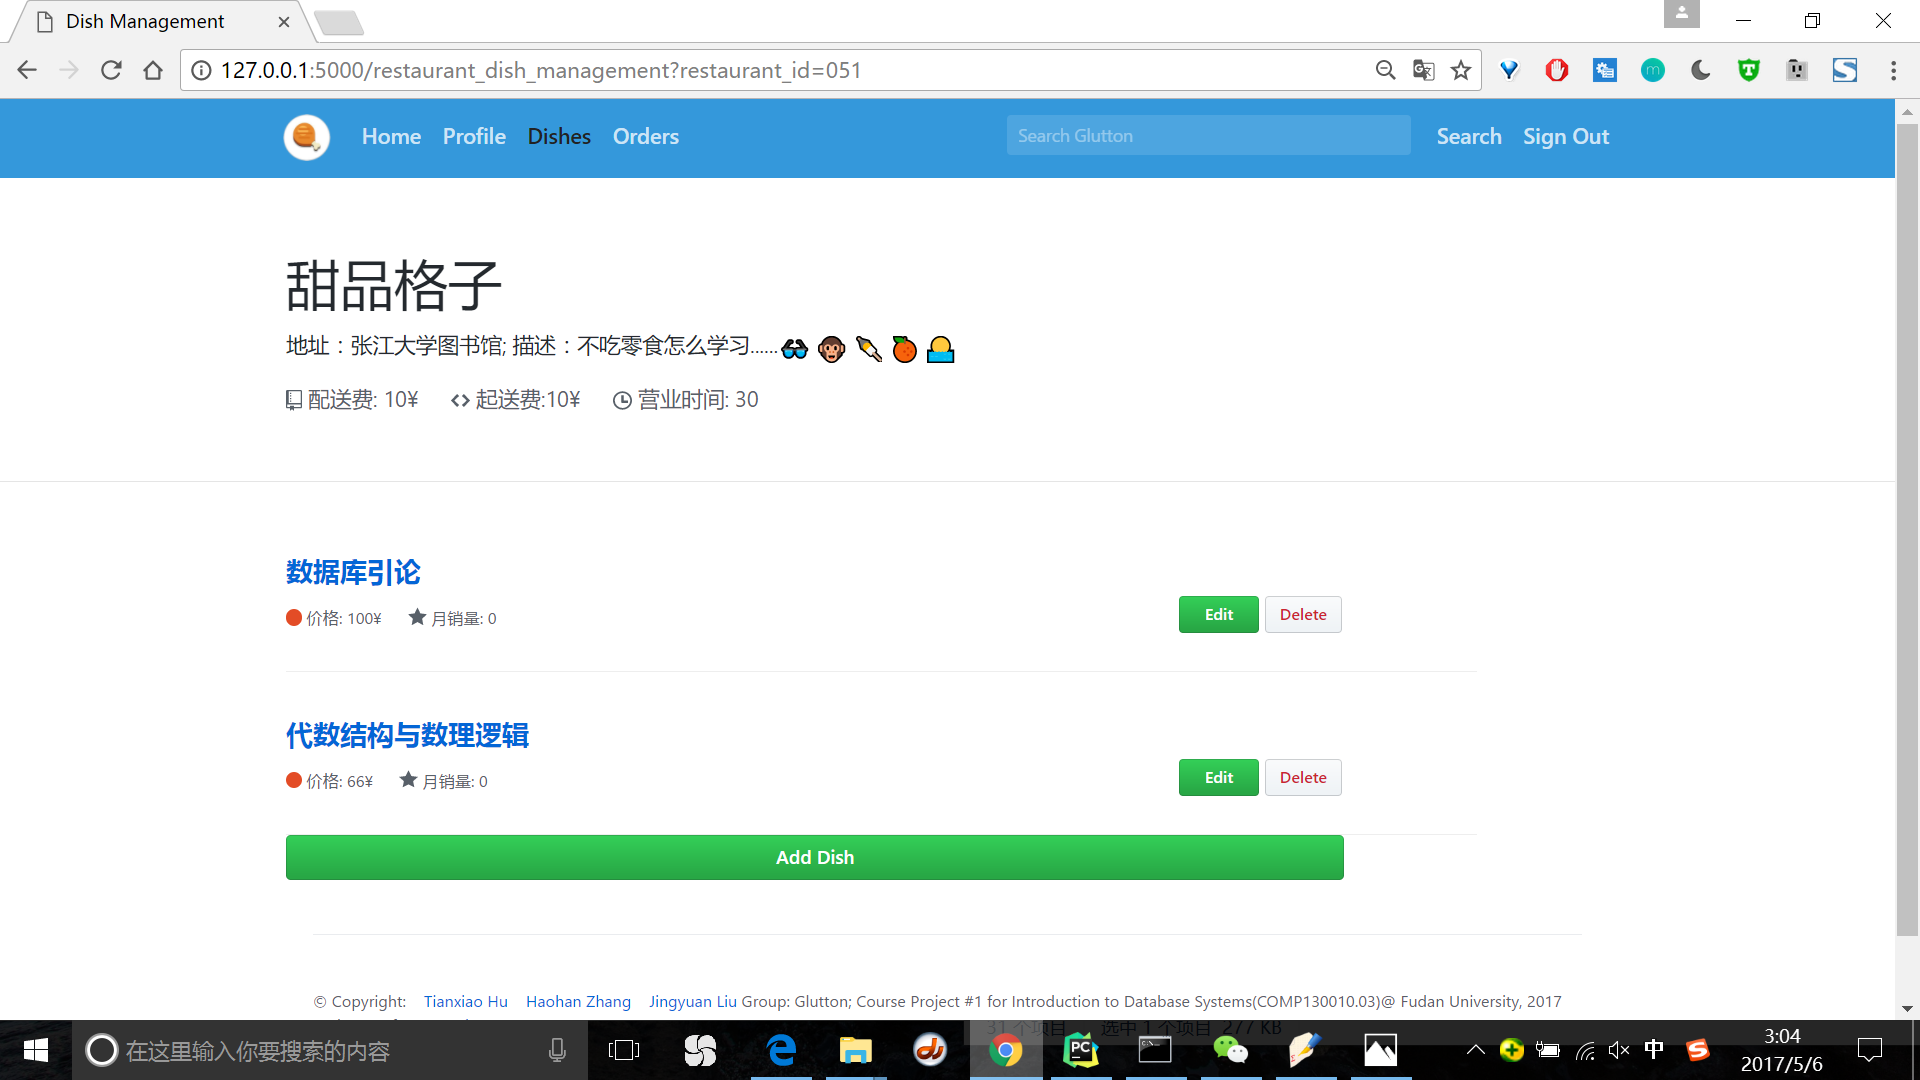
\includegraphics[width=3.2in]{re-dish.jpg}
      \caption{\small{商家查看菜品}}
   \end{minipage}
   \end{figure}
  \item 修改菜品\\
  在菜品管理页面中,点击Edit按钮,可以对菜品名,单价进行修改。
  \begin{figure}[H]
   \begin{minipage}[t]{0.5\linewidth}
    \centering
     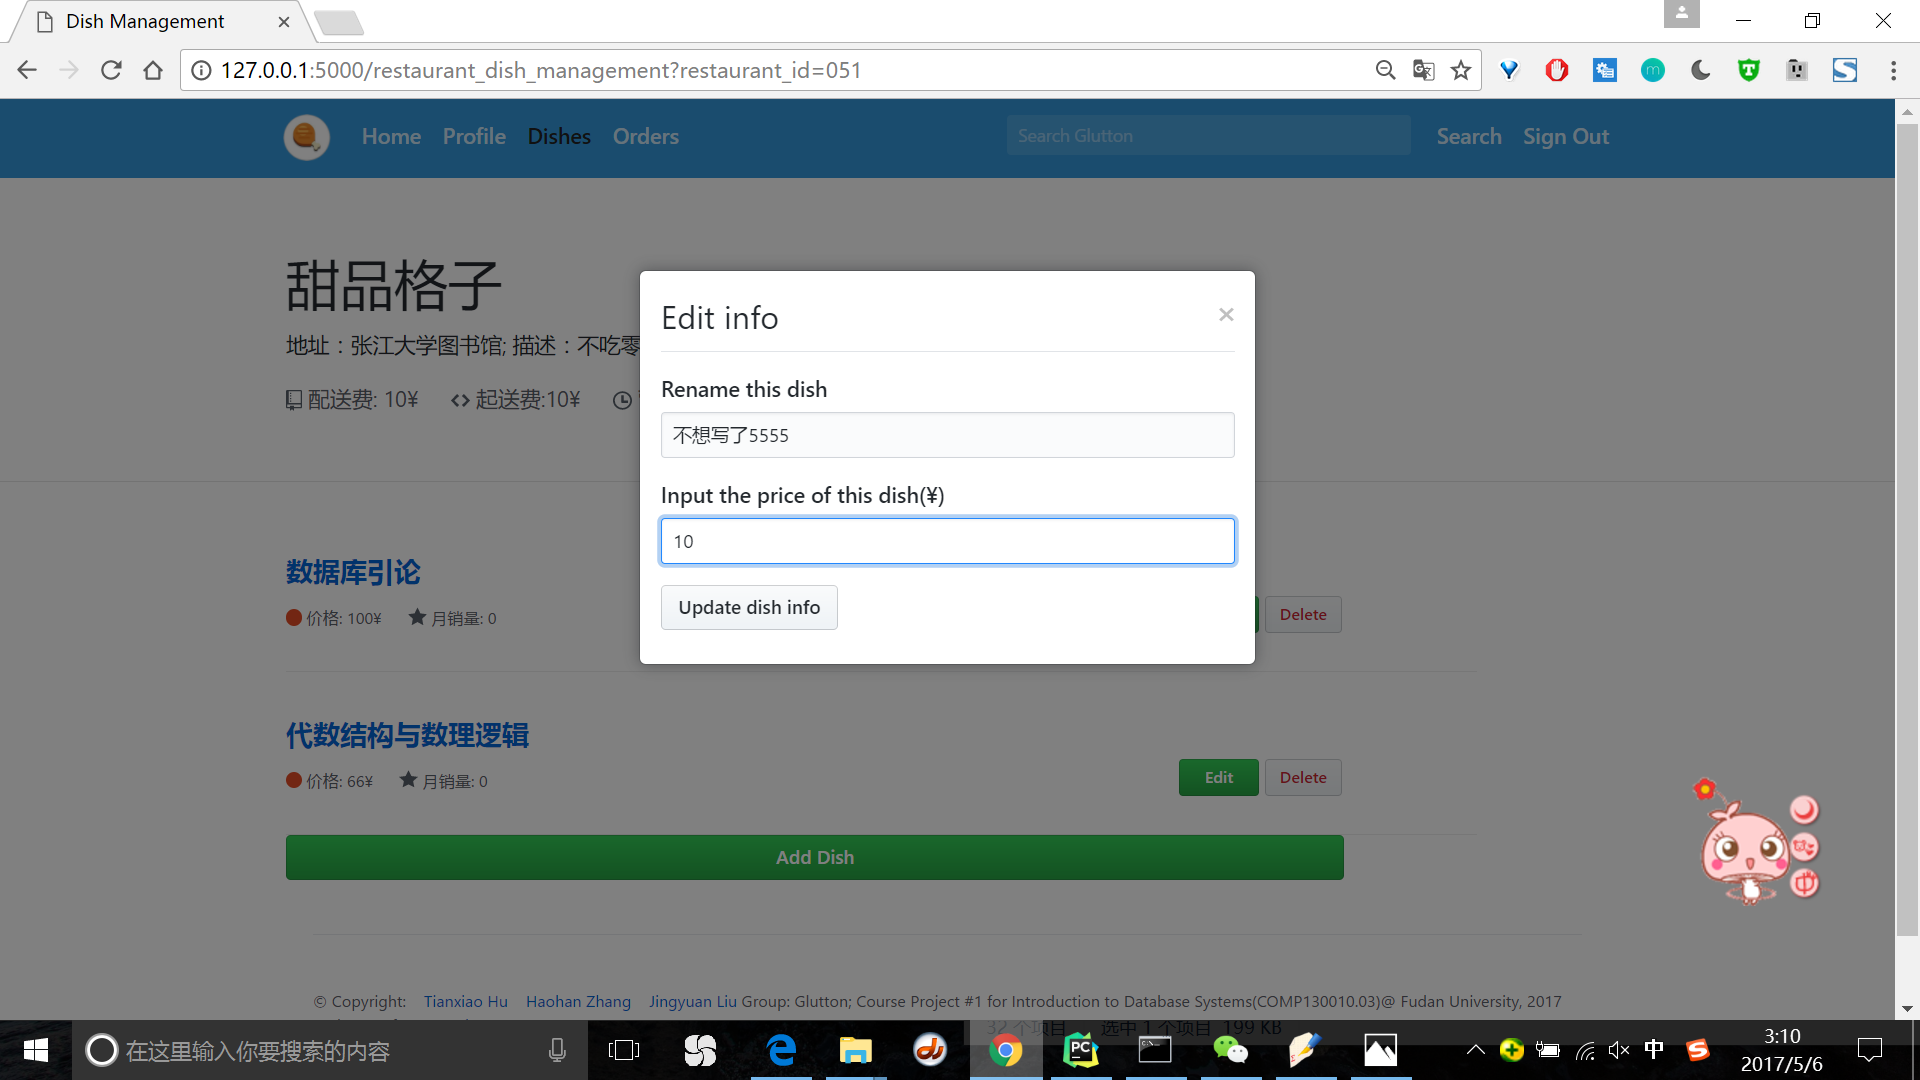
\includegraphics[width=3.2in]{re-update-dish1.jpg}
     \caption{\small{商家修改菜品信息}}
   \end{minipage}
   \begin{minipage}[t]{0.5\linewidth}
    \centering
     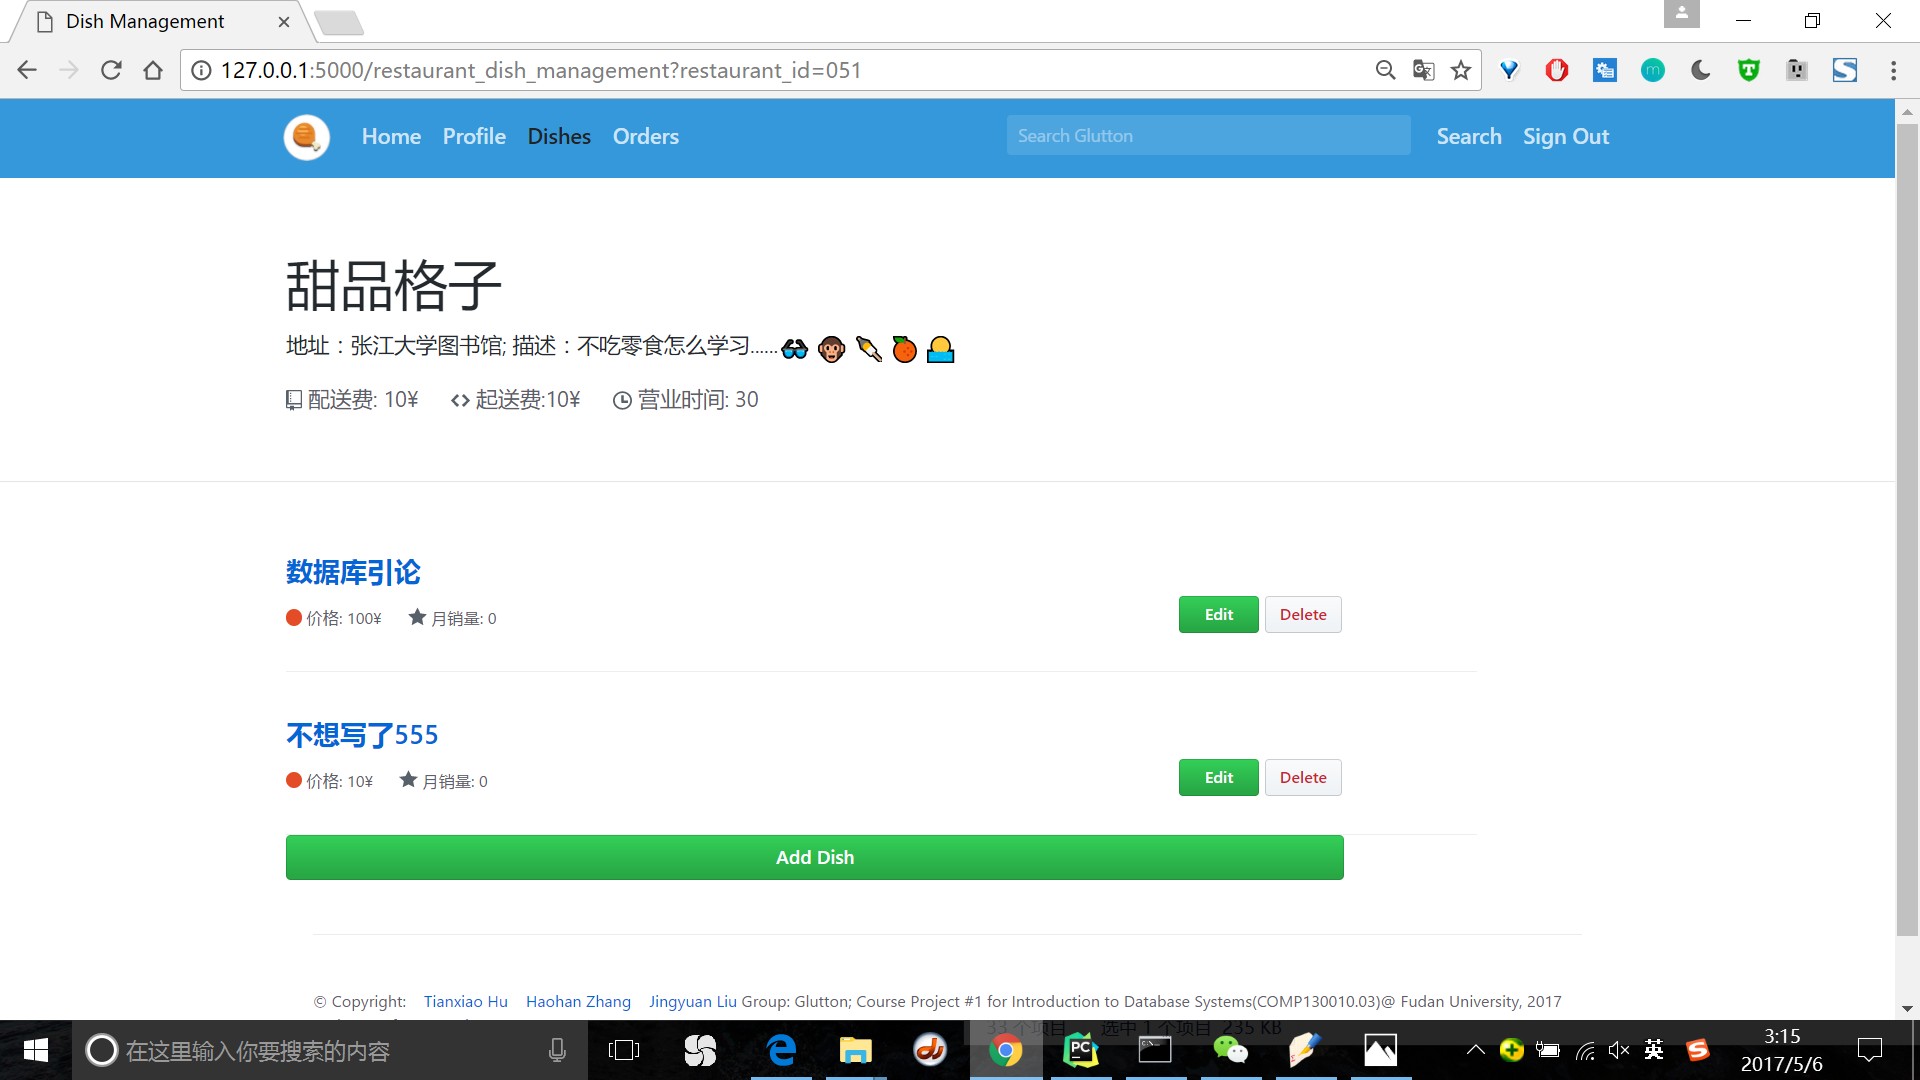
\includegraphics[width=3.2in]{re-update-dish2.jpg}
      \caption{\small{商家修改菜品后}}
   \end{minipage}
   \end{figure}
  \item 删除菜品\\
  在菜品管理页面中,点击Delete按钮,可以对菜品删除。系统会提示是否确定要删除该菜品,确定后,提示菜品删除成功,并跳转到菜品管理页面。
  \begin{figure}[H]
   \begin{minipage}[t]{0.5\linewidth}
    \centering
     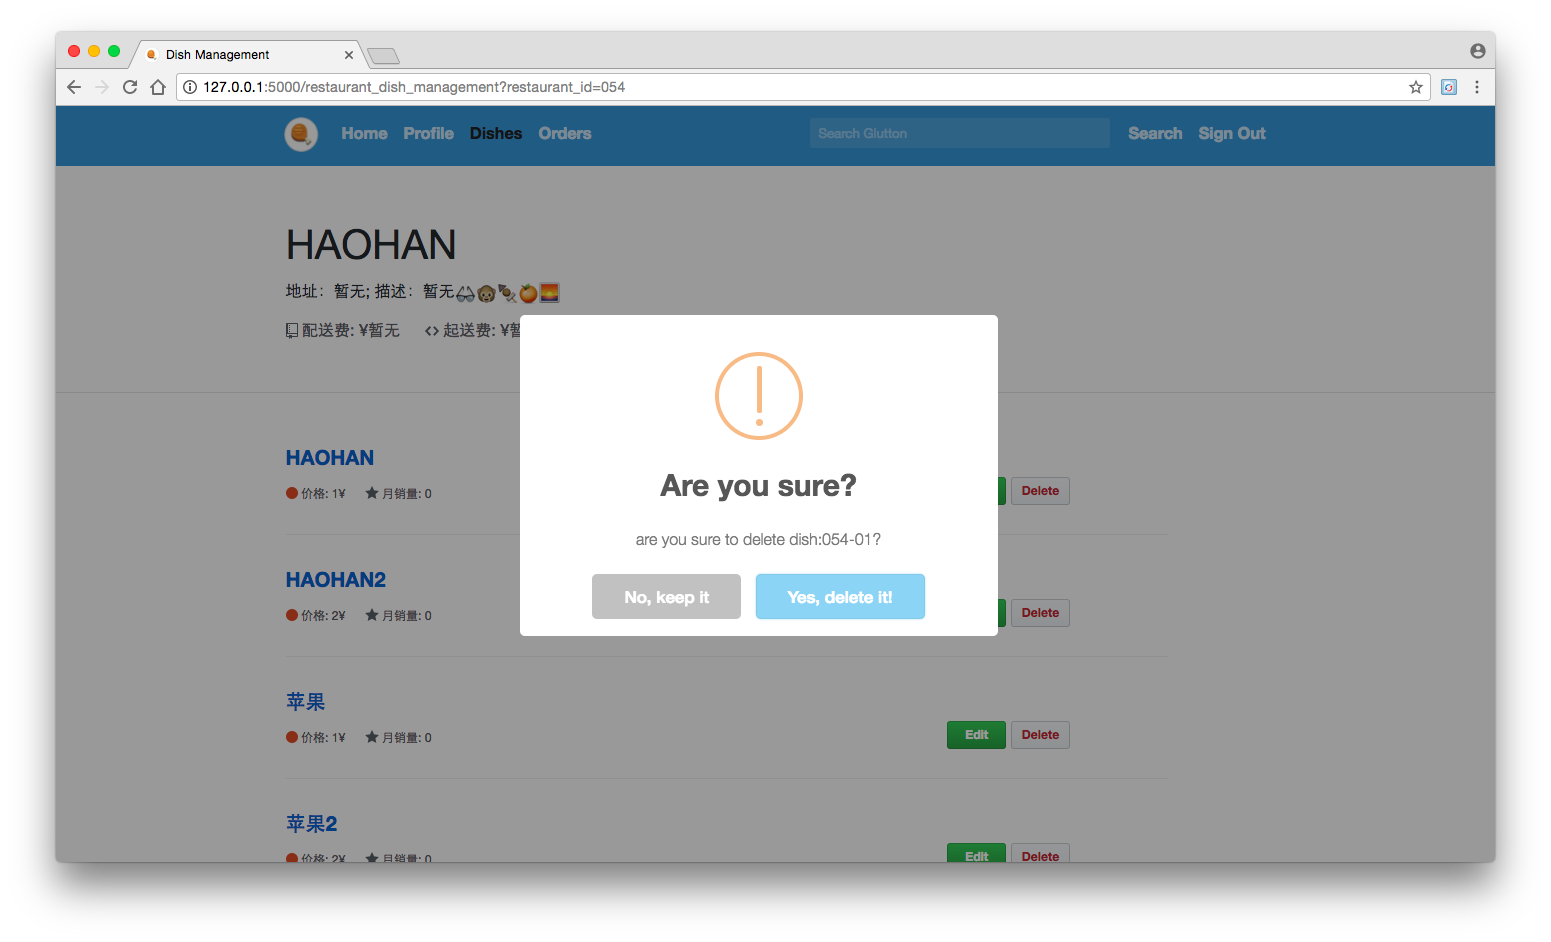
\includegraphics[width=3.2in]{re-delete-dish1.jpg}
     \caption{\small{商家删除菜品}}
   \end{minipage}
   \begin{minipage}[t]{0.5\linewidth}
    \centering
     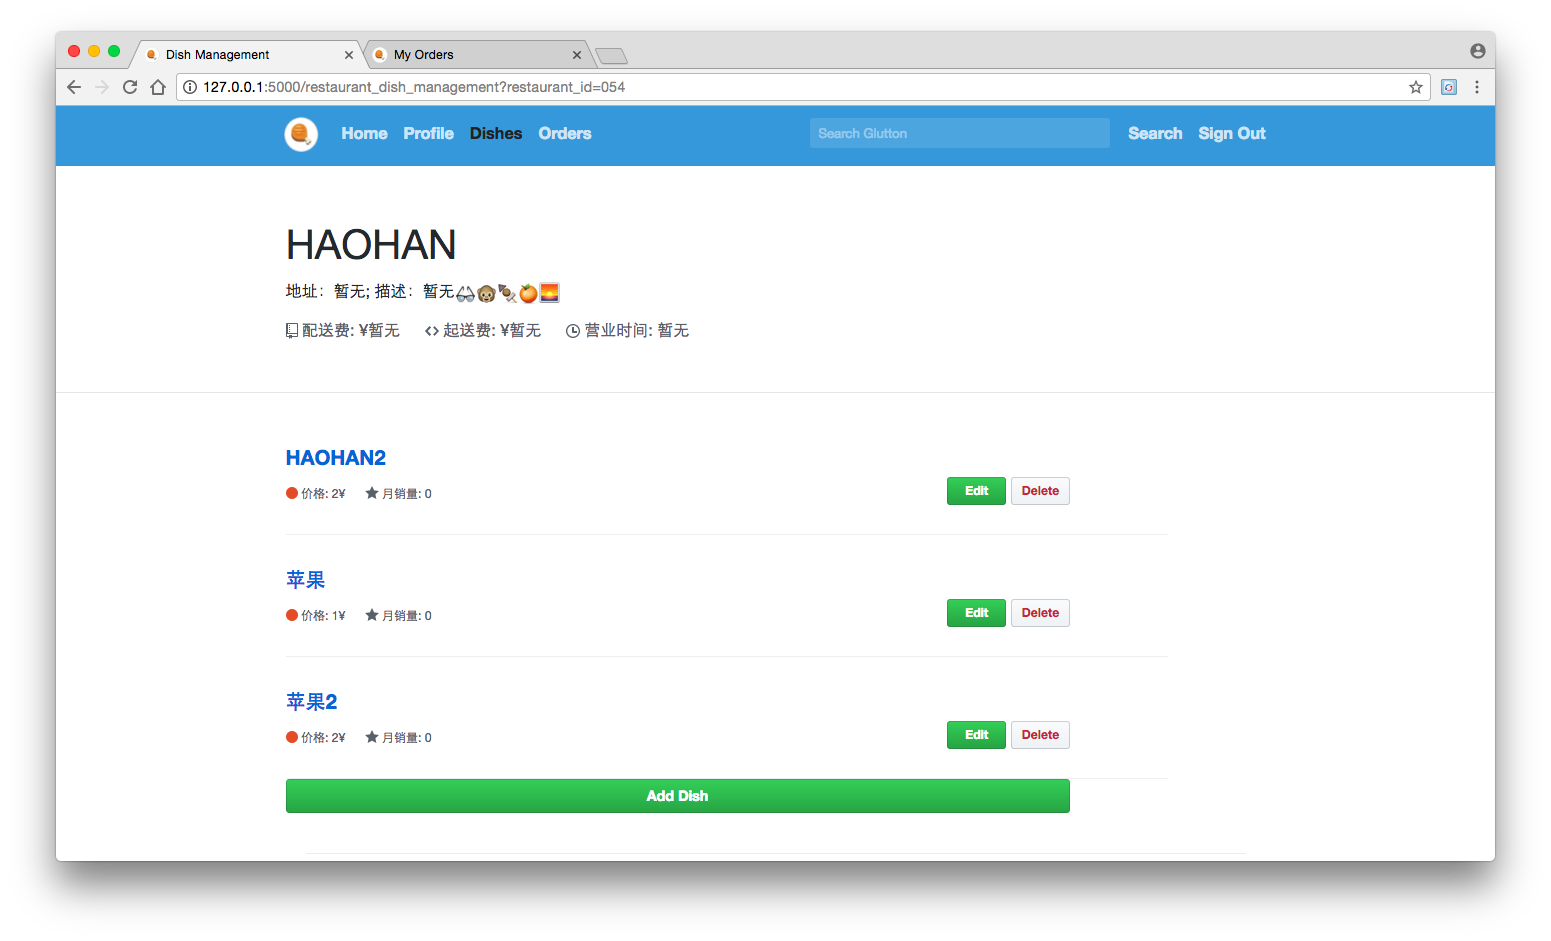
\includegraphics[width=3.2in]{re-delete-dish2.jpg}
      \caption{\small{商家删除菜品后}}
   \end{minipage}
   \end{figure}
  \item 查看商家订单历史\\
  新开的店铺订单信息为空,我们以用户身份登录,下单这家店铺的菜品,可以看到所有订单信息。\\
  我们还可以查看每个订单的评论。
  \begin{figure}[H]
   \begin{minipage}[t]{0.5\linewidth}
    \centering
     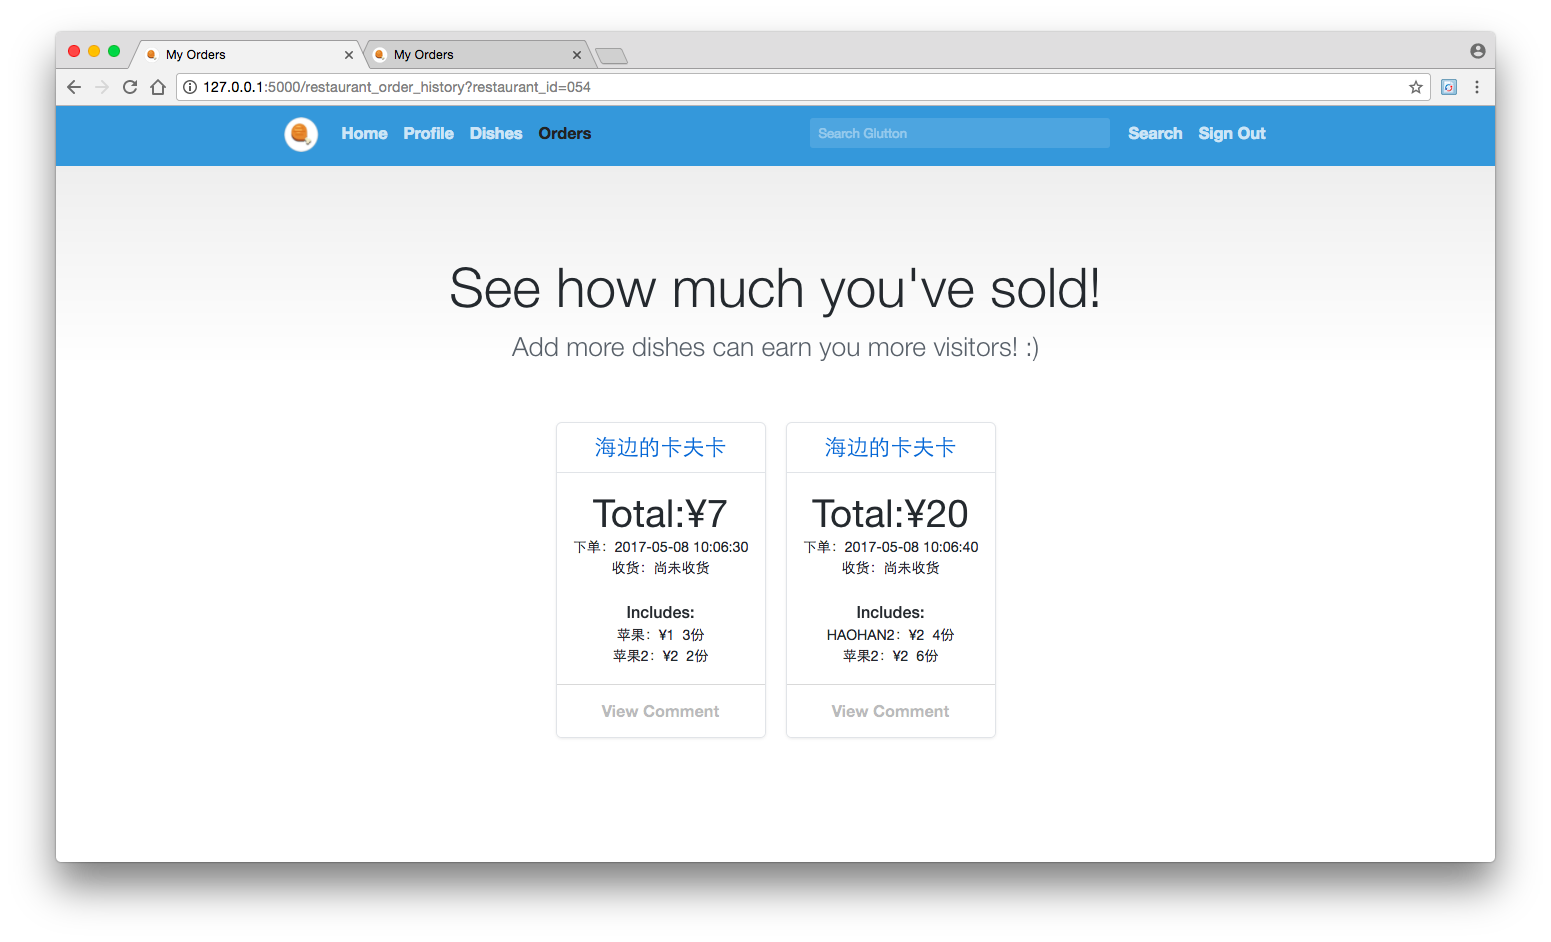
\includegraphics[width=3.2in]{re-order.jpg}
     \caption{\small{商家查看订单历史}}
   \end{minipage}
   \begin{minipage}[t]{0.5\linewidth}
    \centering
     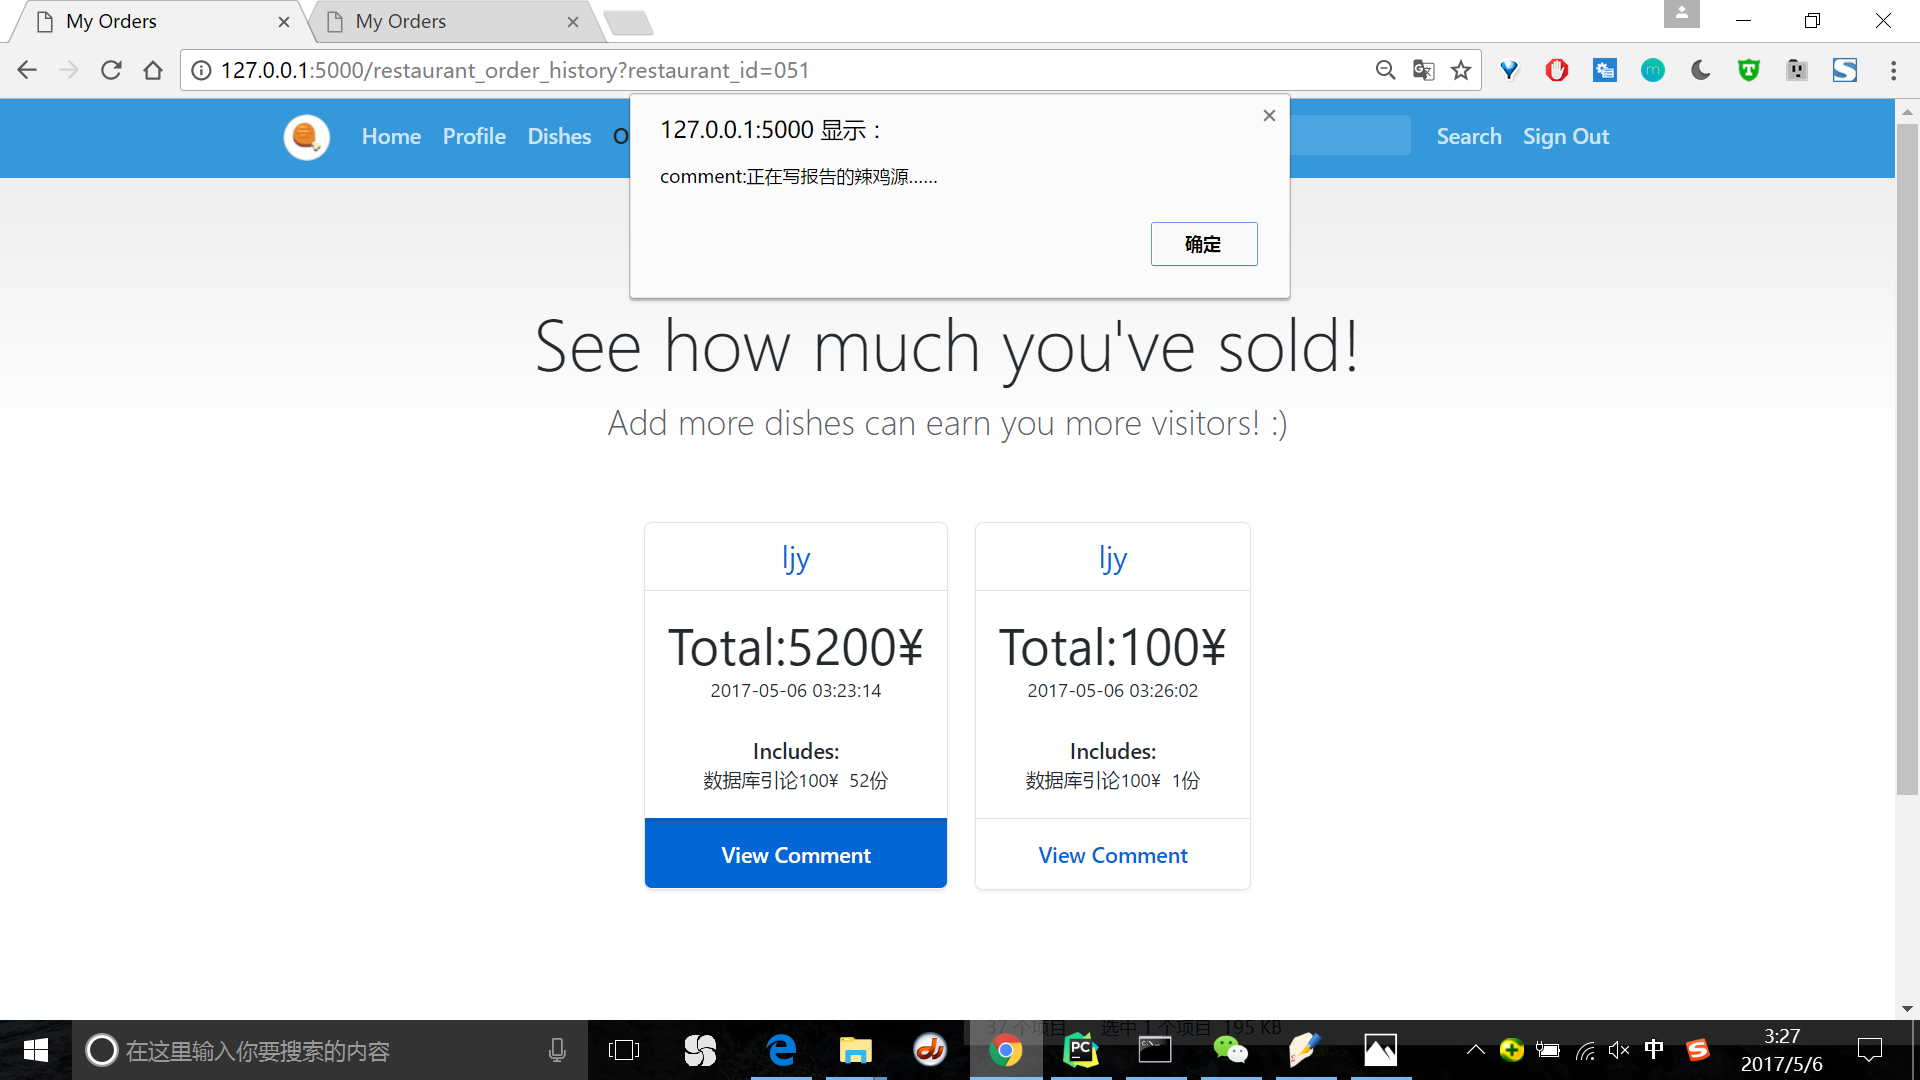
\includegraphics[width=3.2in]{re-order-comment.jpg}
      \caption{\small{商家查看订单评价}}
   \end{minipage}
   \end{figure}
  \end{itemize}

\section{数据库简介}
\subsection{数据库设计}
\begin{itemize}
 \item ER图
  \begin{figure}[H]
   \centering
     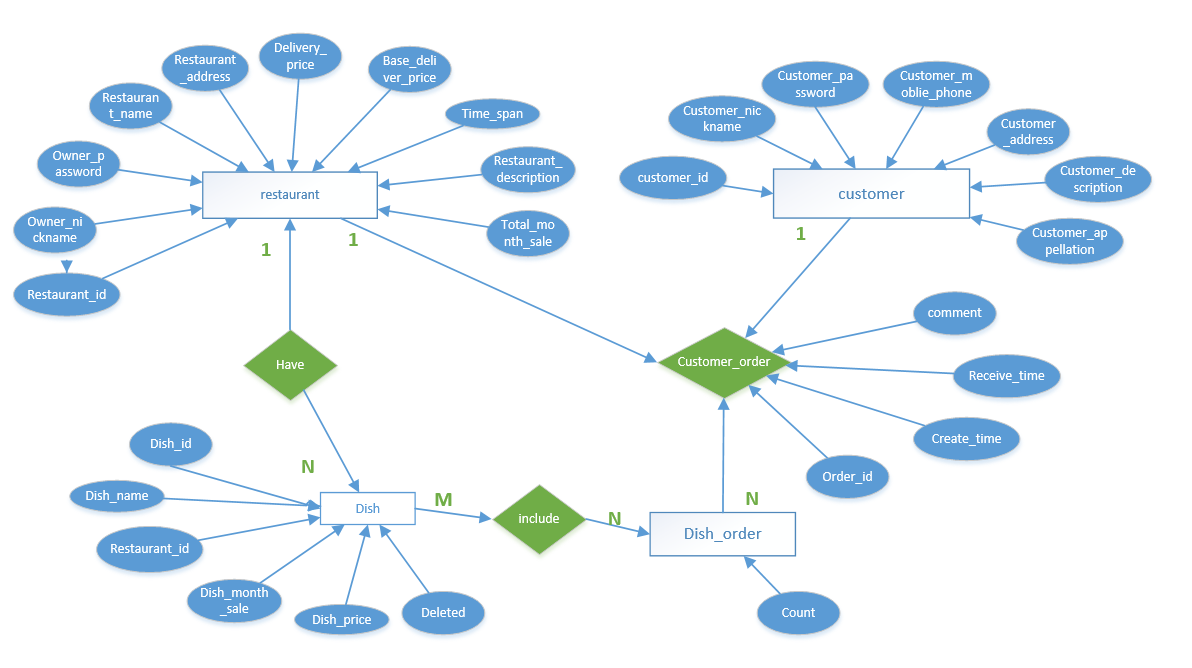
\includegraphics[width=6.50in]{ER.png}
     \caption{\small{数据库ER图}}
  \end{figure}

 \item 关系图
  \begin{figure}[H]
    \centering
     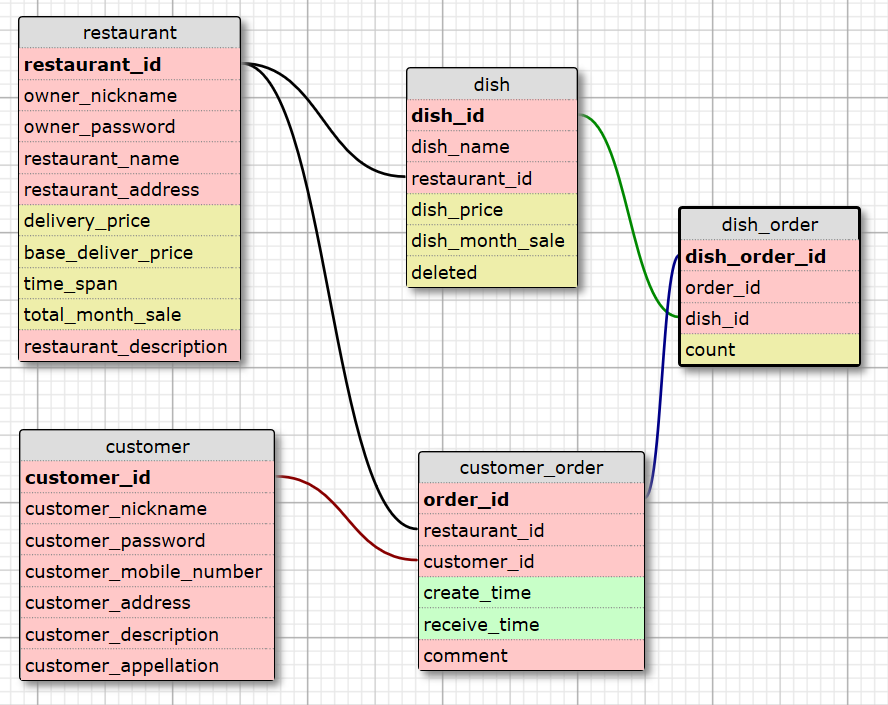
\includegraphics[width=6.5in]{tables.png}
     \caption{\small{数据库表格关系图}}
  \end{figure}
\end{itemize}
\subsection{数据源}
Glutton所用数据来源于外卖平台”饿了么“网站,以复旦大学(张江校区)为中心,选取真实的商家信息作为数据源,保证了数据的真实性和有效性。\\
数据选取以蔡伦路、科苑路、华佗路的商铺为主,涵盖50个商家。每个商家菜品若干,最多为17道菜,最少为4道菜,共393道菜,平均每个商家8道菜。整个数据库包含443条商家及菜品记录。
\subsection{数据库操作:增、删、改、查}
\subsubsection{建表语句}
Glutton数据库共包含5张表:商家表、用户表、菜品表、用户订单表、菜品订单表。
 \begin{itemize}
 \item \textbf{商家表}信息包括:商家号、用户名、密码、商家名、商家地址、配送费、起送价、平均配送时间、营业时间、月销量、商家公告,主键为商家号。
 \begin{lstlisting}
   CREATE TABLE restaurant(
   restaurant_id CHAR(3) NOT NULL,
   owner_nickname CHAR(20) NOT NULL UNIQUE,
   owner_password CHAR(40) NOT NULL,
   restaurant_name CHAR(50) NOT NULL,
   restaurant_address CHAR(100),
   delivery_price DECIMAL(5,2),
   base_deliver_price DECIMAL(5,2),
   time_span SMALLINT,
   open_time  CHAR(20),
   total_month_sale INTEGER,
   restaurant_description CHAR(200),
   PRIMARY KEY(restaurant_id)
   );
\end{lstlisting}
 \item \textbf{用户表}信息包括:用户号、用户名、密码、手机号、收获地址、用户个人描述、用户称呼、用户口味偏好,主键为用户号,其中用户手机号应该是唯一的,加UNIQUE 区分。
      \begin{lstlisting}
   CREATE TABLE customer(
   customer_id CHAR(3) NOT NULL,
   customer_nickname CHAR(20) NOT NULL,
   customer_password CHAR(40) NOT NULL,
   customer_mobile_number CHAR(20) UNIQUE,
   customer_address CHAR(100),
   customer_description CHAR(100),
   customer_appellation CHAR(20),
   customer_avatar CHAR(20) NOT NULL,
   PRIMARY KEY(customer_id)
   );
      \end{lstlisting}
 \item \textbf{菜品表}信息包括:菜品号、菜品名、所属商家号、菜品价格、菜品月销量,主键为菜品号,外键为所属商家号,即可将菜品与商家联系起来。其中,商家删除菜品后,不能影响用户历史订单对这个菜品显示,所以加deleted属性。当商家删除菜品后,deleted为true,该菜品不在商家中显示,而用户历史订单中仍然可以查询到。
     \begin{lstlisting}
   CREATE TABLE dish(
   dish_id CHAR(6) NOT NULL,
   dish_name CHAR(30) NOT NULL,
   restaurant_id CHAR(3) NOT NULL,
   dish_price DECIMAL(5,2) NOT NULL,
   dish_month_sale SMALLINT,
   deleted BOOL,
   PRIMARY KEY(dish_id),
   FOREIGN KEY(restaurant_id)REFERENCES restaurant(restaurant_id)
   );
      \end{lstlisting}
 \item \textbf{用户订单表}信息包括:商家号、用户号、用户订单号、创建时间、收货时间、评论,主键为用户订单号,外键商家号、用户号分别关联商家表和用户表。
     \begin{lstlisting}
   CREATE TABLE customer_order(
   restaurant_id CHAR(3) NOT NULL,
   customer_id CHAR(3) NOT NULL,
   order_id CHAR(3) NOT NULL,
   create_time DATETIME NOT NULL,
   receive_time DATETIME,
   comment CHAR(100),
   PRIMARY KEY(order_id),
   FOREIGN KEY(restaurant_id)REFERENCES restaurant(restaurant_id),
   FOREIGN KEY(customer_id)REFERENCES customer(customer_id)
   );
      \end{lstlisting}
 \item \textbf{菜品订单表}信息包括:菜品订单号、用户订单号、菜品号、菜品数量,主键为菜品订单号,外键用户订单号、菜品号分别关联用户订单表和菜品表。这种设计使一个订单可以表示多个菜品,并减少了数据冗余。
     \begin{lstlisting}
   CREATE TABLE dish_order(
   dish_order_id CHAR(4) NOT NULL,
   order_id CHAR(4) NOT NULL,
   dish_id CHAR(6) NOT NULL,
   count SMALLINT NOT NULL ,
   PRIMARY KEY(dish_order_id),
   FOREIGN KEY(order_id)REFERENCES customer_order(order_id) ON DELETE CASCADE,
   FOREIGN KEY(dish_id)REFERENCES dish(dish_id)
   );
      \end{lstlisting}
 \end{itemize}

\subsubsection{插入语句}
利用INSERT语句向数据库中插入商家、菜品、用户、订单信息。
  \begin{itemize}
   \item 建立数据库时的数据插入
    \begin{lstlisting}
   //插入商家信息
   INSERT INTO restaurant VALUES
   ('001','restaurant1','password','学城粥铺','上海市浦东新区张江镇华佗路572 号',2,0,45,'09:00-23:00',743,
   '需要米饭的亲们,可以在商品里面点哦,我们的炒菜是不配米饭的,
    除了商务套餐和盖浇饭以外,敬请谅解');
   //插入菜品信息
   INSERT INTO dish VALUES
   ('002-10','伴鸡伴虾堡','002',19,7);
    \end{lstlisting}
   \item 应用期间的数据插入
    \begin{lstlisting}
   //用户在创建账号时插入:用户ID,用户名,用户密码,用户手机号,用户口味偏好
   INSERT INTO customer VALUES
   ('%s', '%s', '%s', '%s', NULL, NULL, NULL, '1');
   //用户在创建订单时,插入用户订单信息:商家号、用户号、用户订单号、创建时间
   INSERT INTO customer_order VALUES
   ('%s', '%s', '%s', '%s', NULL, NULL);
   //用户在创建订单时,插入菜品订单信息:菜品订单号、用户订单号、菜品号、菜品数量
   INSERT INTO dish_order VALUES
   ('%s', '%s', '%s', '%d');
   //商家在新开一家店铺时,插入店铺信息:商家号、用户名、密码、商家名
   INSERT INTO restaurant VALUES
   ('%s', '%s', '%s', '%s', NULL, NULL, NULL, NULL, NULL, NULL, NULL);
   //商家可以插入新的菜品信息:菜品号、菜品名、商家号、菜品价格、月销量及价格
   INSERT INTO dish VALUES
   ('%s','%s', '%s', '%f', '%d', '%d')
   //……
    \end{lstlisting}
  \end{itemize}

\subsubsection{查询语句}
   利用SELECT语句查询商家、菜品、订单信息。
  \begin{itemize}
   \item 商家
     可以查看自己店铺的菜品和订单,并可以选择以一定的顺序(如菜品月销量,订单创建时间等)列表显示。
    \begin{lstlisting}
    //选择用户订单
	SELECT customer_order.customer_id, customer_order.order_id, customer_order.create_time, customer_order.receive_time, customer_order.comment
	FROM customer_order WHERE restaurant_id = '%s'
	//选择与用户订单对应的菜品订单
	SELECT dish.dish_name, dish.dish_price, dish_order.count
	FROM dish, dish_order, customer_order
	WHERE customer_order.order_id = dish_order.order_id
	AND dish_order.dish_id = dish.dish_id
	AND customer_order.order_id = '%s'
    \end{lstlisting}
   \item 用户
     用户可以查询某一店铺、菜品,按照某一顺序查看所有商家、菜品,查询自己的订单历史记录等,部分代码如下:
    \begin{lstlisting}
   //用户注册时按照手机号查找用户,看是否已经注册
   SELECT * FROM customer WHERE customer_mobile_number = '%s'
   //用户登录时按照手机号对应用户密码是否正确
   SELECT customer_password FROM customer WHERE customer_id = '%s'
   //用户进入个人主页时查找用户个人信息
   SELECT * FROM customer WHERE customer_id = '%s'
   //用户模糊查询某商家
   SELECT * FROM restaurant WHERE restaurant_name LIKE '%%s%';
   //用户模糊查询某道菜品
   SELECT dish_id, dish_name, dish.restaurant_id, dish_price, dish_month_sale,restaurant_name FROM dish, restaurant
   WHERE dish_name LIKE '%%s%'
   AND dish.restaurant_id = restaurant.restaurant_id AND NOT deleted;
   //用户按照最低起送价顺序查询商家
   SELECT * FROM restaurant
   WHERE restaurant_name LIKE '%%s%'
   ORDER BY base_deliver_price
   //用户按照最高月销量顺序查询商家
   SELECT * FROM restaurant
   WHERE restaurant_name LIKE '%%s%'
   ORDER BY total_month_sale DESC
   //用户按照最低价格顺序查询菜品
   SELECT dish_id, dish_name, dish.restaurant_id, dish_price, dish_month_sale,restaurant_name
   FROM dish, restaurant WHERE dish_name LIKE '%%s%' AND dish.restaurant_id = restaurant.restaurant_id AND NOT deleted
   ORDER BY dish_price
   //用户按照最高月销量顺序查询菜品
   SELECT dish_id, dish_name, dish.restaurant_id, dish_price, dish_month_sale, restaurant_name FROM dish, restaurant
   WHERE dish_name LIKE '%%s%' AND dish.restaurant_id = restaurant.restaurant_id AND NOT deleted
   ORDER BY dish_month_sale DESC
   //用户进入商家后返回商家的全部菜品信息
   SELECT  dish_id, dish_name, dish.restaurant_id,dish_price, dish_month_sale
   FROM dish, restaurant
   WHERE dish.restaurant_id = restaurant.restaurant_id
   AND restaurant.restaurant_id = '%s' AND NOT deleted
    \end{lstlisting}
  \end{itemize}

\subsubsection{更改语句}
   利用update语句修改商家、菜品、用户、订单等信息。
  \begin{itemize}
   \item 商家
   \begin{lstlisting}
   //商家修改店铺信息:商家名、商家地址、配送费、起送价,营业时间,店铺公告
   UPDATE restaurant SET restaurant_name = '%s', restaurant_address = '%s',
   delivery_price = '%s', base_deliver_price = '%s', open_time = '%s',
   restaurant_description = '%s' WHERE restaurant_id = '%s';
   //商家修改密码
   UPDATE restaurant SET owner_password = '%s' WHERE restaurant_id = '%s'
   //商家修改菜品信息
   UPDATE dish SET dish_price = '%f', dish_name = '%s'  WHERE dish_id = '%s';
   \end{lstlisting}
   \item 用户
   \begin{lstlisting}
   //用户修改个人信息:用户名,用户地址,用户描述
   UPDATE customer SET customer_nickname = '%s', customer_address = '%s',
          customer_description = '%s', customer_appellation = '%s'
   WHERE customer_id = '%s'
   //用户修改密码
   UPDATE customer SET customer_password = '%s' WHERE customer_id = '%s';
   //用户修改个人头像
   UPDATE customer SET customer_avatar = '%s' WHERE customer_id = '%s';
   //用户收到订单
   UPDATE customer_order SET receive_time = '%s' WHERE order_id = '%s';
   //用户评论订单
   UPDATE customer_order SET comment = '%s' WHERE order_id = '%s';
   \end{lstlisting}
  \end{itemize}

\subsubsection{删除语句}
    使用DELETE语句实现显式删除,UPDATE 语句结合菜品deleted属性实现隐式删除。
   \begin{itemize}
    \item 商家删除菜品
      此处采用隐式删除的方式,对于被删除的菜品,deleted属性被置为true,在商家列表中不再显示,且用户不能再查询到该菜品。但在用户历史订单中仍可以看到该菜品,这种设计更符合实际情况。
       \begin{lstlisting}
   UPDATE dish SET deleted = 1 WHERE dish_id = '%s'
       \end{lstlisting}
    \item 用户删除订单
      采用级联删除的方法,对于被删除的用户订单customer\_order,删除这一条元组的同时,在菜品订单dish\_order 表中同时删除以该订单为外键的菜品订单。
       \begin{lstlisting}
   //SQLite中foreign_keys默认为off,采用级联删除时需要手动改为on
	PRAGMA foreign_keys = ON
	DELETE FROM customer_order WHERE order_id = '%s'
        \end{lstlisting}
   \end{itemize}

\end{document}